\documentclass[11pt, oneside]{article}   	% use "amsart" instead of "article" for AMSLaTeX format
\usepackage[a4paper, total={6.27in, 9.69in}]{geometry}

\geometry{letterpaper}                   		% ... or a4paper or a5paper or ... 
%\geometry{landscape}                		% Activate for for rotated page geometry
\usepackage[parfill]{parskip}    		% Activate to begin paragraphs with an empty line rather than an indent
\usepackage{graphicx}				% Use pdf, png, jpg, or eps§ with pdflatex; use eps in DVI mode
%\usepackage{multicol}								% TeX will automatically convert eps --> pdf in pdflatex	
\usepackage{amssymb}
\usepackage{afterpage}
\usepackage{natbib}
\usepackage{hyperref}
\usepackage{placeins}
\usepackage{subcaption}

\title{
\textbf{Agent-based models and the mathematical equations that describe them}}
\author{Amy Hurford*, James Watmough, Joany Mari\~{n}o, Anne McLeod, and Christina Prokopenko \\
\ *email: ahurford@mun.ca}
\date{}

\begin{document}
\maketitle
\tableofcontents

\newpage
\section{Agent-Based Models}
Agent-based models (ABMs) consider discrete individuals (agents), and are usually stochastic and spatially explicit. Formulating ABMs is intuitive for ecologists with a good knowledge of the intrinsic and extrinsic factors affecting their study organisms, although the value of simplifying assumptions and mathematical approximations can be underappreciated. Complex agent-based models are difficult to interpret and analyze: the stochastic ABM needs to be run many times and the results may consist of many variables, making it difficult to know which aspects to emphasize. When many variables interact, it can be difficult to build hypotheses as to which aspects of the organism's biology are useful to explain the model's results.

The goal of this workshop is to alleviate some of these challenges by showing how specifically formulated ABMs can be approximated by mathematical equations which are easier to comprehensively analyze. In Section \ref{sec:SSA}, we explain how to formulate an ABM that is stochastic and with discrete individuals, so that it can be approximated with a system of ordinary differential equations. This first example is not spatially explicit and assumes that all individuals are equally likely to interact with one and other. In Section \ref{sec:PA} we provide an example of a spatially explicit model where individuals are resident on a lattice and can interact with their nearest neighbours. This spatially explicit lattice-based ABM is approximated by a system of ordinary differential equations that describes the frequency of adjacent patches on the lattice with a particular status, for example, the frequency of adjacent patches that are both occupied by individuals of different epidemiological statuses. Section \ref{sec:AR} describes additional reading. In the Appendix (Section \ref{sec:Appendix}), we provide some explanations of the software choices and installation.

The software requirements to complete this workshop are described in Section \ref{sec:software}.

\section{A non-spatial predator-prey model}\label{sec:SSA}
\subsection{The Gillespie Stochastic Simulation Algorithm}
In this section, we consider a non-spatial ABM; however, despite the lack of space, this ABM is still more realistic than an ordinary differential equation, in that the ABM is stochastic and that individuals are discrete. We will use Gillespie's Stochastic Simulation Algorithm \citep{Gillespie} to formulate our ABM. The ABM that we formulate will be approximated by the predator-prey equations with logistic birth rate for sheep and a type II functional response. Our ABM assumes only two species are present: the number of sheep (prey) is $S$, and the number of wolves (predators) is $W$. The model assumes the following events:

\begin{description} 
\item[$E_1:$] Each sheep will reproduce to generate, on average, $b(1-S/K)$ new sheep per year, where $K$ is the carrying capacity.
\item[$E_2:$] Each sheep will die of natural causes at an average rate of $d_S$ deaths per year. This rate may be greater than 1, which would imply that, on average, sheep die of natural causes in less than a year.
\item[$E_3:$] Each sheep will die due to wolf predation at an average rate of $cW/(1+cS)$ predation events per year.
\item[$E_4:$] Each wolf will reproduce in proportion to the rate of sheep predation, where the proportionality constant is $\epsilon$, which is unitless, and should sensibility be less than 1 due to energy loss up the food chain. 
\item[$E_5:$] Each wolf will die of natural causes at an average rate of $d_W$ deaths per year.
\end{description}
 
It should be noted that the model does not track each wolf's sheep consumption and link individual-level sheep consumption to that wolf's reproduction. This individual-level bookkeeping is unnecessary because the model is not spatial and all wolves are identical.\footnote{Given that there are no individual-level variables, it could be argued that this example is not truly an agent-based model. None-the-less, this example is a good beginner exercise to help understand the algorithms that are used later for examples where each individual has associated individual-level characteristics.} Across the wolf population there is a distribution of the number of births. Predation events are not assigned to a particular wolf, but if it is easier to conceptualize, it is possible to regard the wolves with higher than average sheep consumption also with having higher than average reproduction. This conceptualization is possible because all wolves are identical.

This description of the Gillespie algorithm is based on (\citealt{Gillespie}; see also Section 5.1.1 Law of Mass Action in \citealt{Muller}). We define the following notation:

\begin{table}[htp]
\begin{center}
\begin{tabular}{ll}
$\mu$ & an index for each event \\
$E_\mu$ & description of the event indexed as $\mu$ \\
$M$ & the total number of events described by the model\\
$a_\mu$ & the rate associated with the the $\mu^{th}$ event\\
$\alpha_0$ & $= \sum_{\mu=1}^M a_\mu$ i.e., the sum of all the rates $\alpha_\mu$ \\
$\mu_i$ & a stochastic realization of the index for the event that occurred on the i$^{th}$ iteration of the code. \\
$\tau_i$ & a stochastic realization of the time that the event $\mu_i$ occurred.\\
\end{tabular}
\end{center}
\label{default}
\end{table}%

Therefore, for our predator-prey ABM as described above, in Gillespie's notation, $\mu \in \{1,2,3,4,5\},$ $M=5$,

\[\vec{E} = \left[\begin{array}{c} \mbox{sheep birth} \\ \mbox{sheep natural mortality} \\ \mbox{sheep predation mortality} \\ \mbox{wolf birth} \\ \mbox{wolf natural mortality} \end{array} \right], \qquad \mbox{and} \qquad \vec{a} = \left[\begin{array}{c} b S\left(1-\frac{S}{K}\right) \\ d_S S \\ \frac{c SW}{1+cS} \\ 
 \frac{\epsilon c SW}{1+cS} \\ d_W W \end{array} \right], \] 

where the elements of the vectors are $\vec{E} = [E_1, E_2, E_3, E_4, E_5]^T$ and $\vec{a} = [a_1, a_2, a_3, a_4, a_5]^T$. The sum of the rates for all events is $a_0 = bS(1-S/K) + d_SS + cSW/(1+cS) + \epsilon cWS/(1+cS) + d_W W$.

Following the reasoning outlined in \cite{Gillespie}, assuming that the time to the next event is exponentially distributed, then
%
\begin{equation}\label{eq:taui}
\tau_i = \frac{1}{a_0}\log \left(\frac{1}{r_{1,i}} \right) \qquad \mbox{where $r_{1,i} \sim U[0,1]$},
\end{equation}
%
where  $r_{1,i} \sim U[0,1]$ means that $r_{1,i}$ is random variable drawn from a uniform distribution defined over the interval from 0 to 1. The event that occurs is determined as,
%
\begin{equation}\label{eq:mui}
\mu_i = \min_k\sum_{j=1}^{k} a_j> a_0 r_{2,i} \qquad \mbox{where $r_{1,i} \sim U[0,1]$}, 
\end{equation}
%
where equation \ref{eq:mui} is a re-written version of equation 21b from \cite{Gillespie}). Equation \ref{eq:mui} can be understood by considering a number line form $0$ to $a_0$ that is divided up into subintervals with lengths corresponding to the rates of their associated events (recall that $a_0$ is the sum of all the rates); then, $a_0r_{2,i}$ is a random point on the line used to determine the corresponding event. The cumulative sum (equation \ref{eq:mui}) defines the end of the subintervals for the event indexed by $k$.

The description of the event, $E_{\mu_i}$, determines how the values of the state variables, $S(t)$ and $W(t)$ are updated. For example, if $\mu_i = 1$ then a sheep is born and the number of sheep increases by 1:
%
\[ S(t+\tau_i) = S(t) + 1\]
%
The other state variable changes are:
\[ \begin{array}{ll}
S(t+\tau_i) = S(t) - 1 & \mbox{for } \mu_i = 2, 3 \\
W(t+\tau_i) = W(t) + 1 & \mbox{for } \mu_i = 4 \mbox{ and } \\
W(t-\tau_i) = W(t) - 1 & \mbox{for } \mu_i = 5. \\
\end{array}
\]

Implemented in this way the ABM is approximated by the predator-prey equations,
%
\begin{eqnarray}\label{eq:PP1}
\frac{dS}{dt} & = & bS\left(1-\frac{S}{K}\right) - d_S S - \frac{c SW}{1+cS}, \\
\frac{dW}{dt} & = &  \frac{\epsilon c SW}{1+cS} - d_W W.\label{eq:PP2}
\end{eqnarray}
%
These equations assume a type II functional response with handling time set to 1.

\subsection{Code files}

\begin{description}
\item[Wolf Sheep SSA.nlogo] A Netlogo program that implements the Gillespie algorithm as described above.
\item[Wolf\underline{ }Sheep\underline{ }Analysis.R] An R script that imports the results of \texttt{Wolf Sheep SSA.nlogo} and numerically solves the system of ordinary differential equations (equations \ref{eq:PP1}-\ref{eq:PP2}).
\item[RosMac2019-08-13.R] An R script that makes figures by calling to \texttt{Rosenzweig-MacArthurSSA.R}. \texttt{Rosenzweig-MacArthurSSA.R} uses the package \texttt{GillespieSSA} to simulate the stochastic process and has other precoded models available.
\end{description}

\subsubsection*{Instructions}
\begin{enumerate}
\item Open \texttt{Wolf Sheep SSA.nlogo} and click the purple \texttt{setup} button. 

\begin{figure}[!ht]
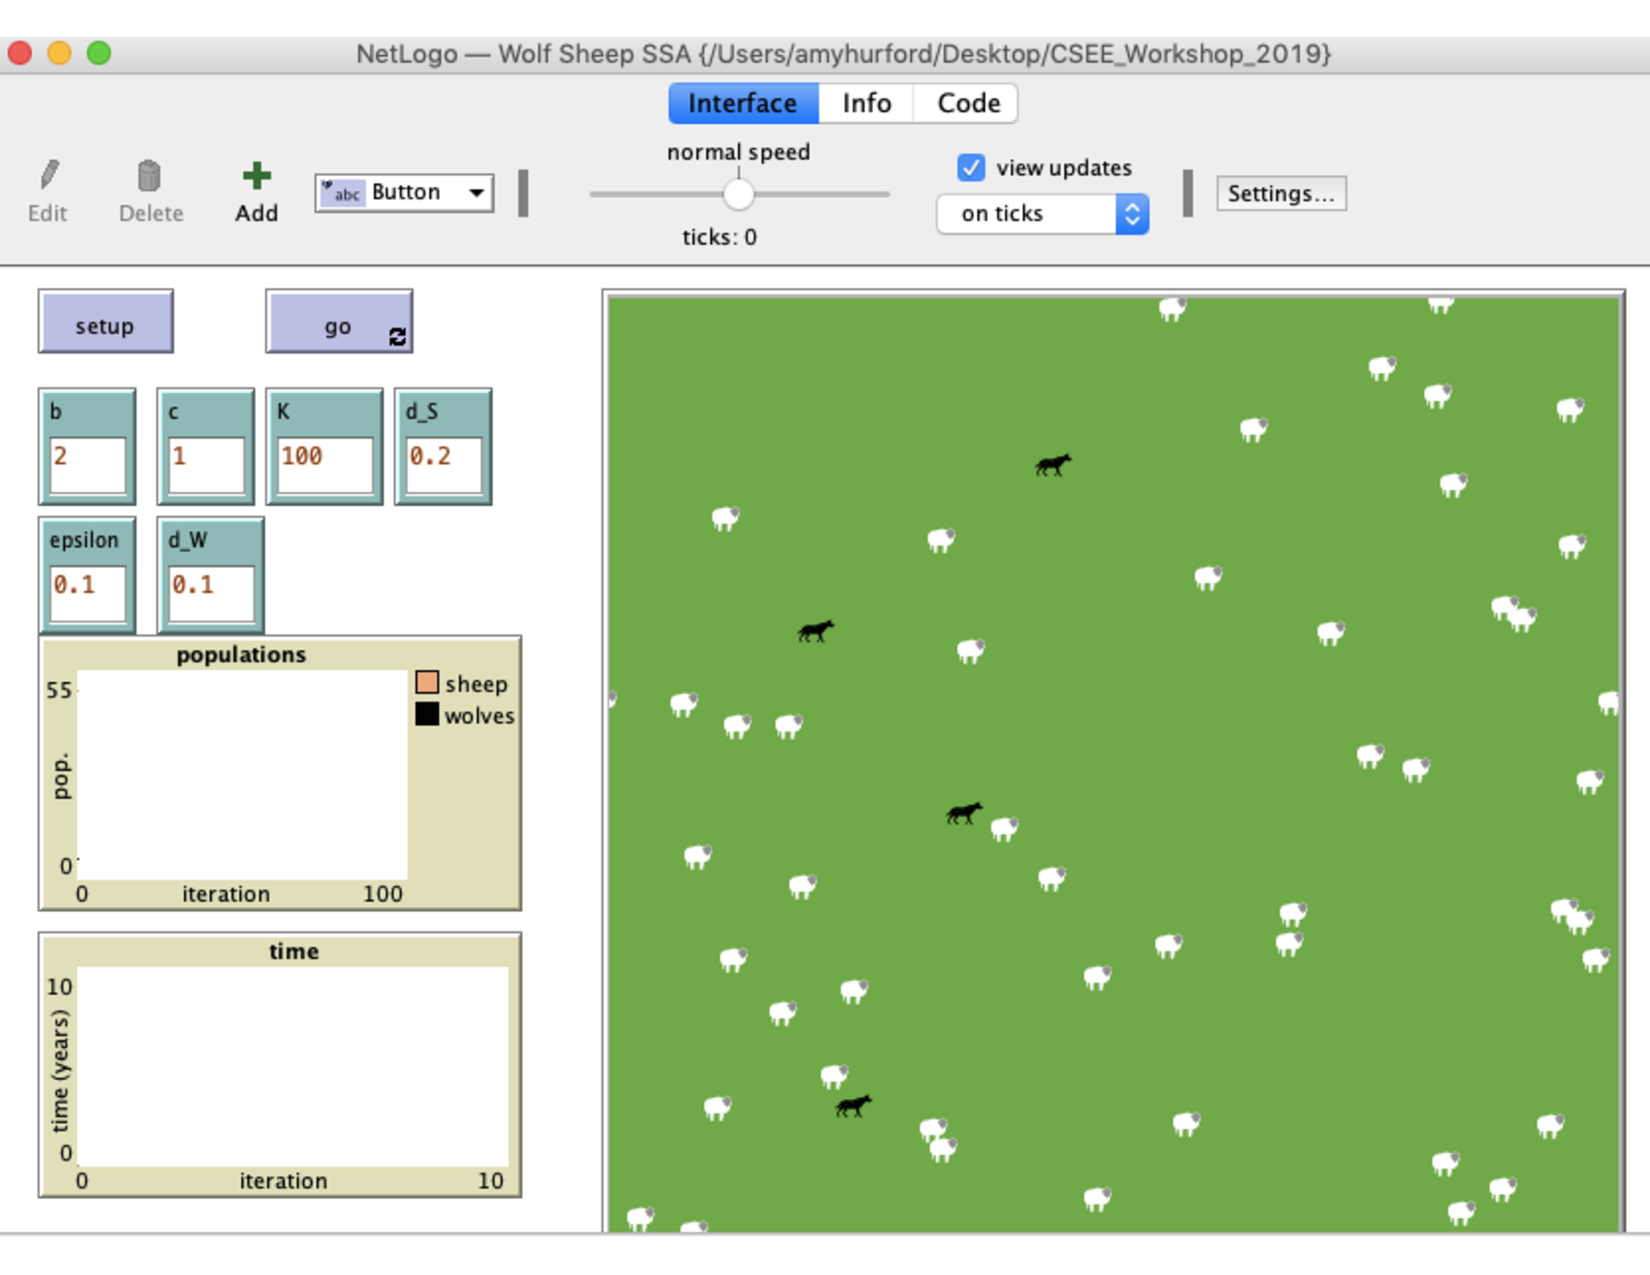
\includegraphics[height=6cm]{setup}
\end{figure}

\item Click the purple \texttt{go} button. The simulation should begin running. Click \texttt{go} again to stop it. The plots track: (1) the number of sheep and wolves (y-axis) and the iteration of the code (x-axis), and (2) time (y-axis) and the iteration of the code (x-axis).

\begin{figure}
\centering
\begin{minipage}{.5\textwidth}
  \centering
  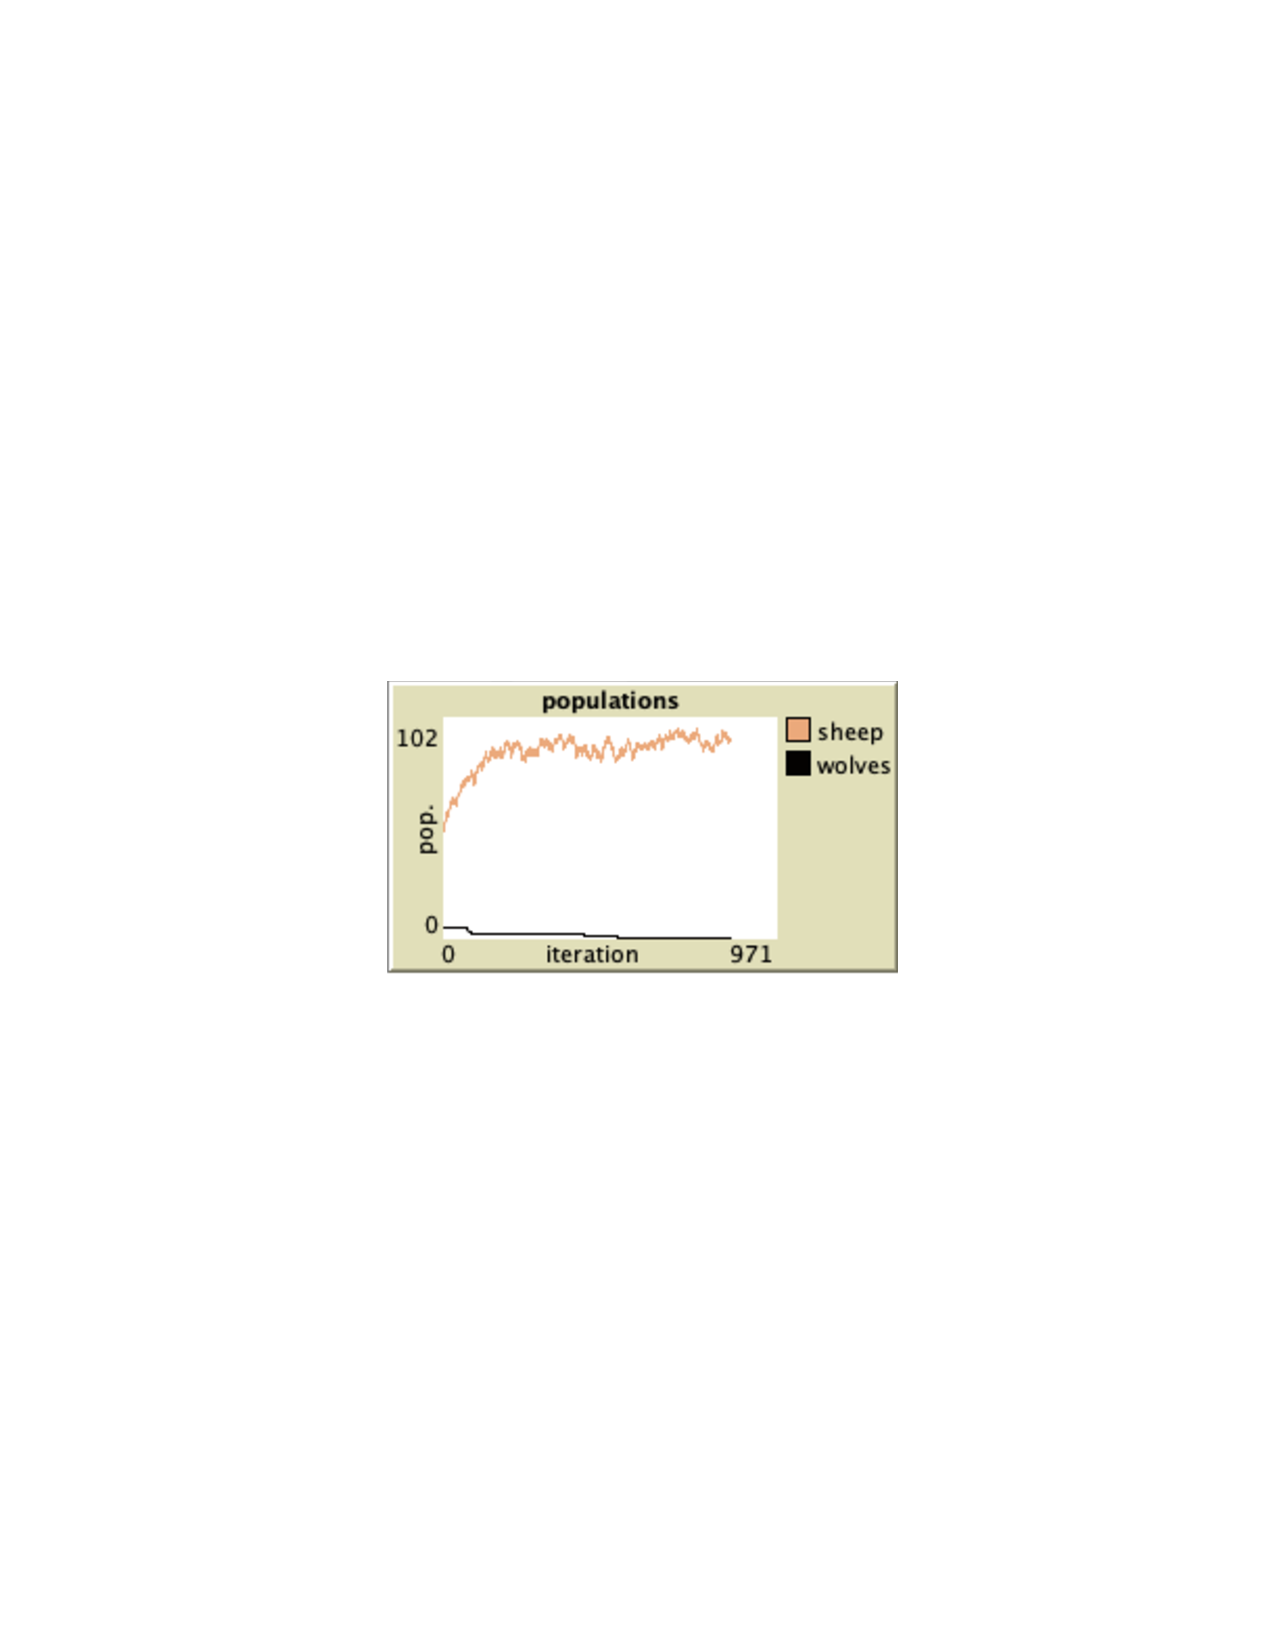
\includegraphics[width=.8\linewidth]{populations}
\end{minipage}%
\begin{minipage}{.5\textwidth}
  \centering
  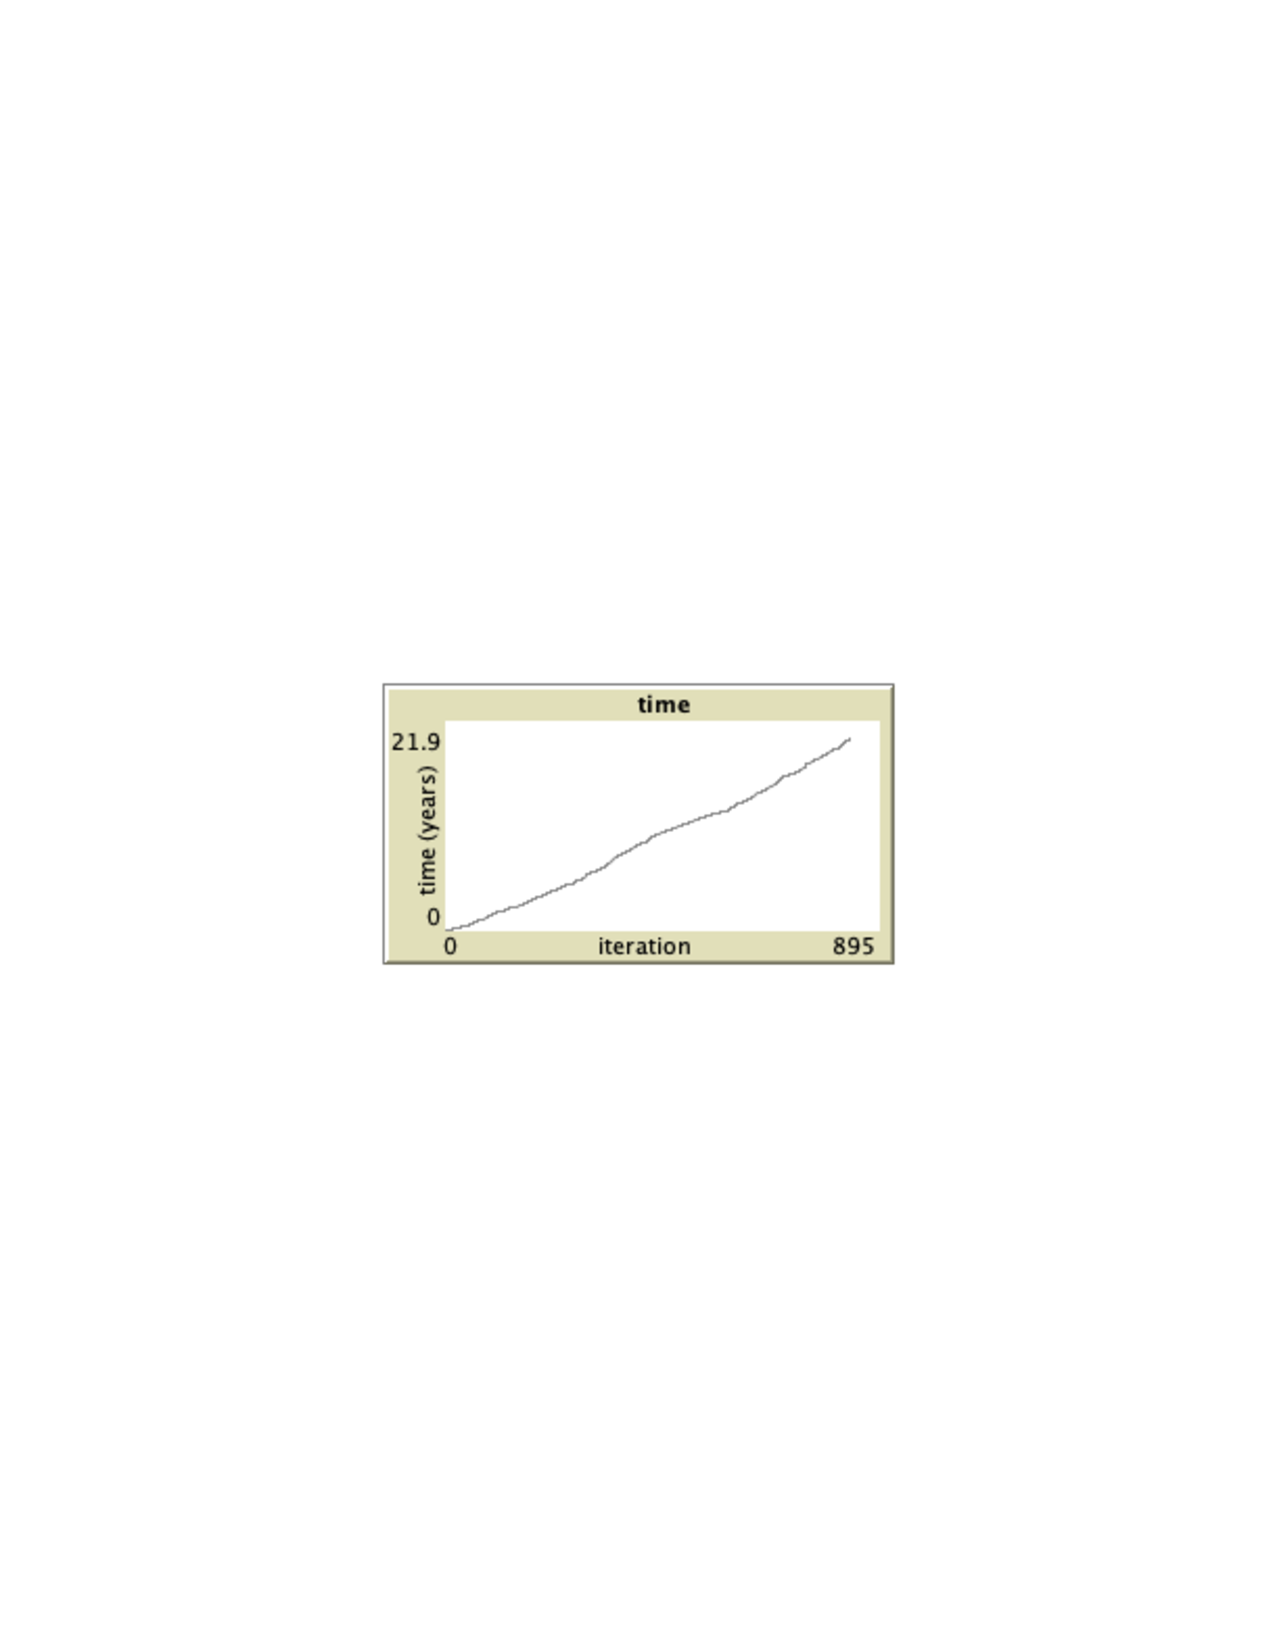
\includegraphics[width=.7\linewidth]{time}
\end{minipage}
\end{figure}
\FloatBarrier

\item You can change the parameters and re-run the simulation.

\begin{figure}[!ht]
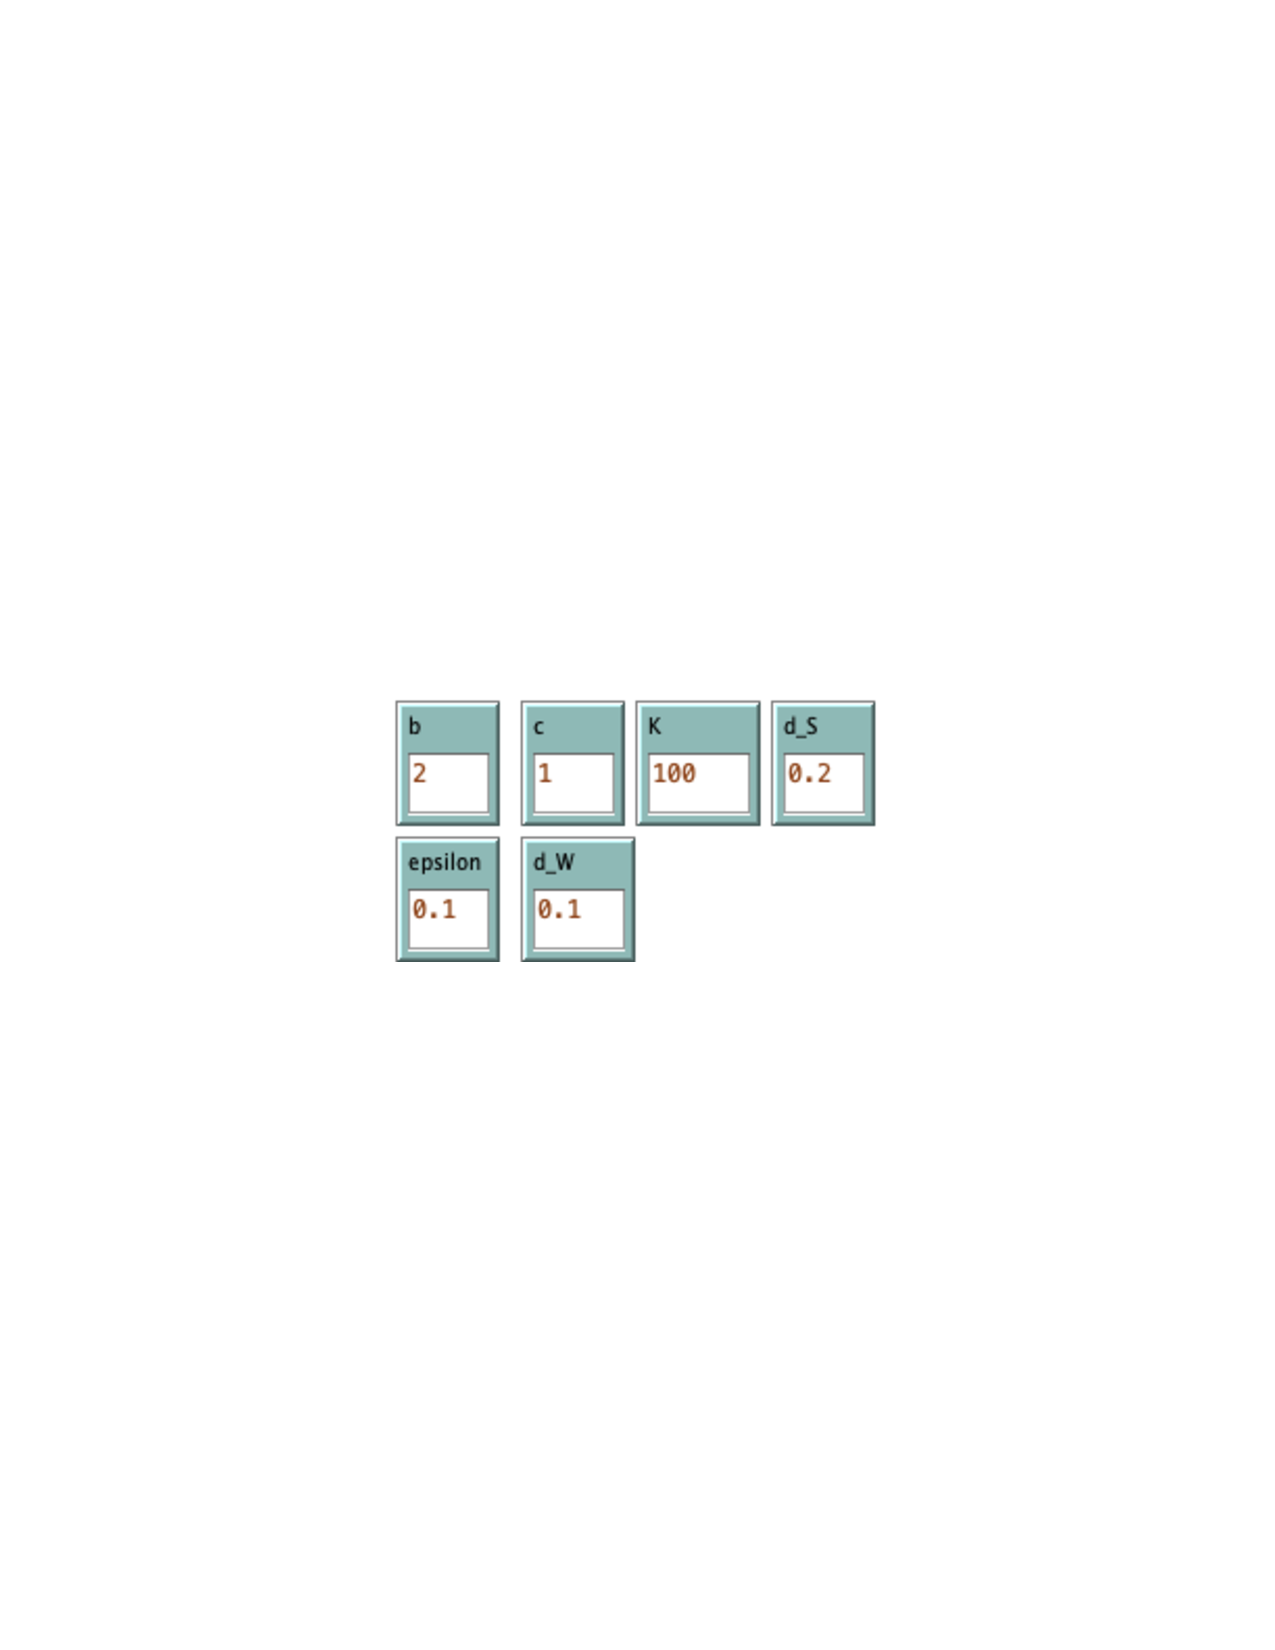
\includegraphics[height=3cm]{parameters}
\end{figure}

\item Now consider the top middle/right of your Netlogo screen. You have the option to uncheck `view updates': this will speed up the results of your simulation. There are also three options: `Interface', `Info', and `Code'. Explore these different views.

\begin{figure}[!ht]
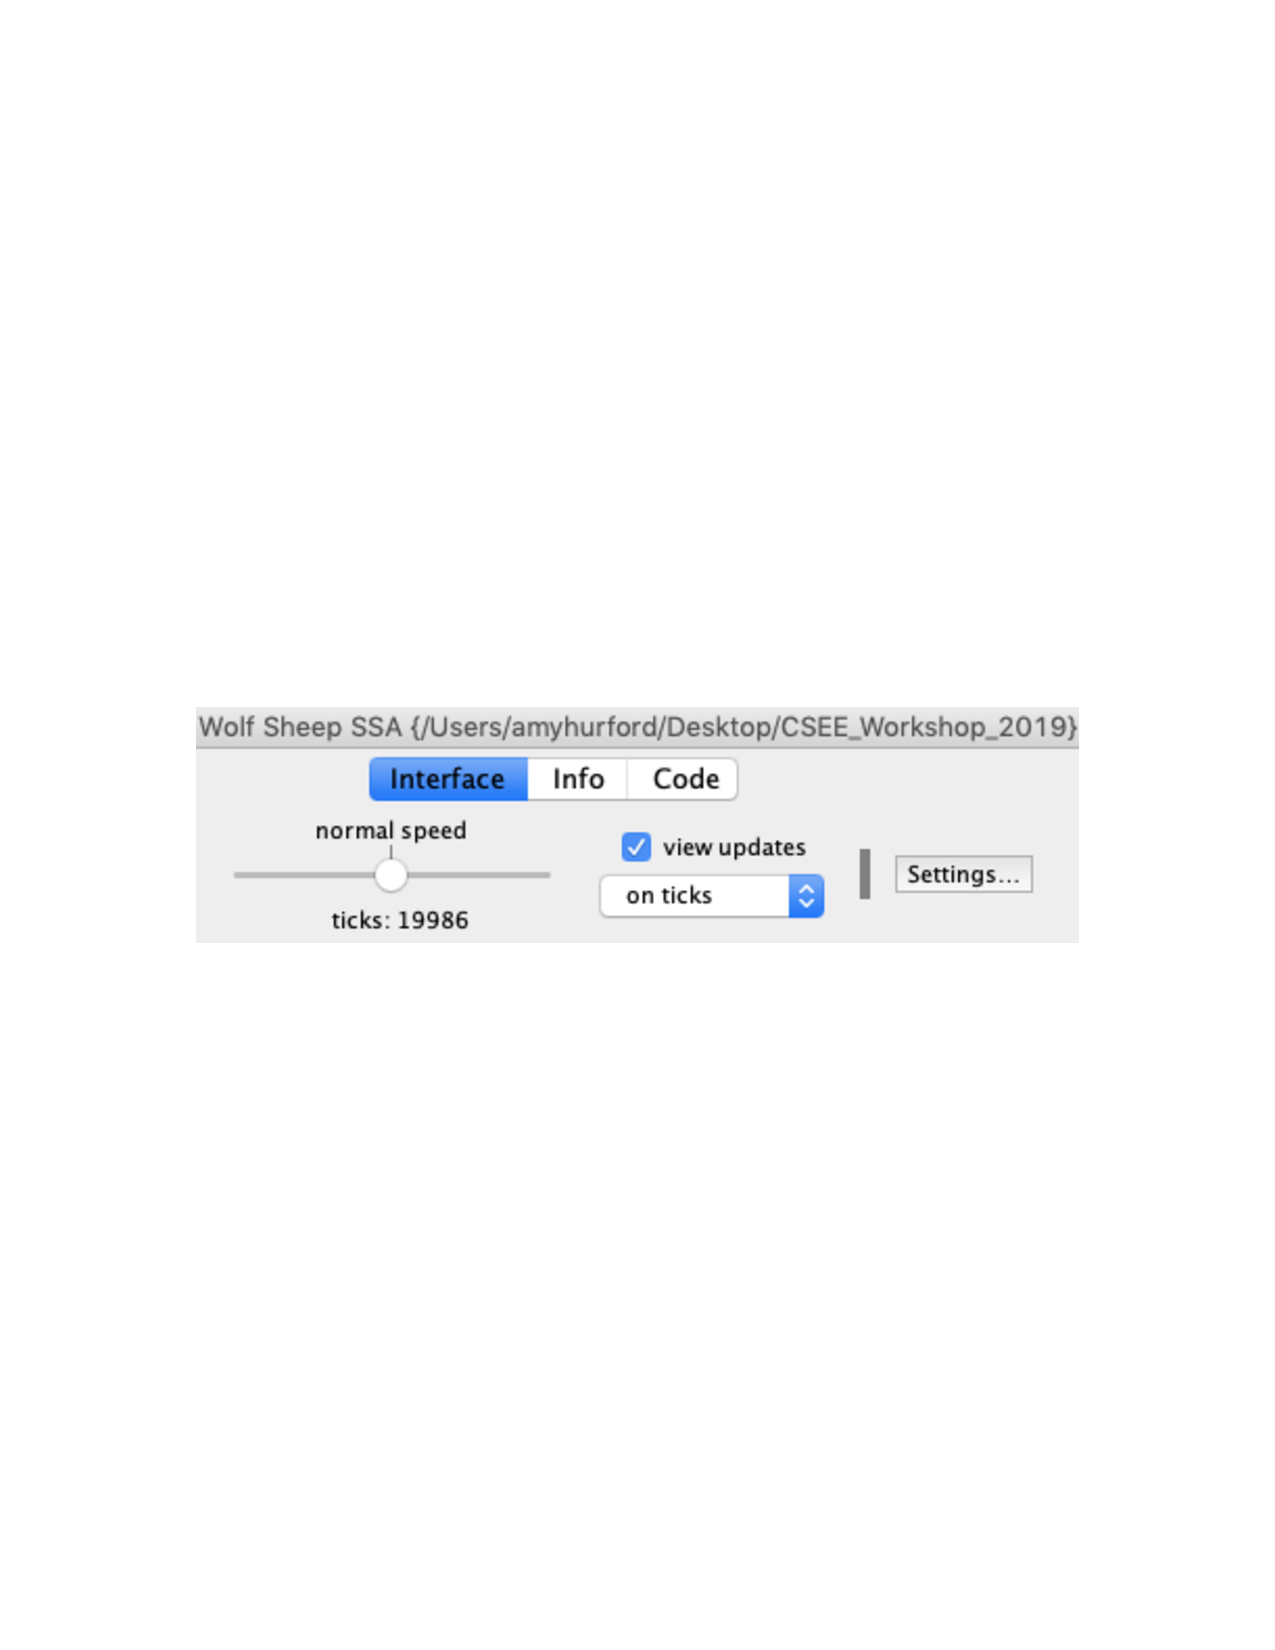
\includegraphics[height=2cm]{top}
\end{figure}

\item In the `Code' view you can identify the lines that end the code:

\begin{figure}[!ht]
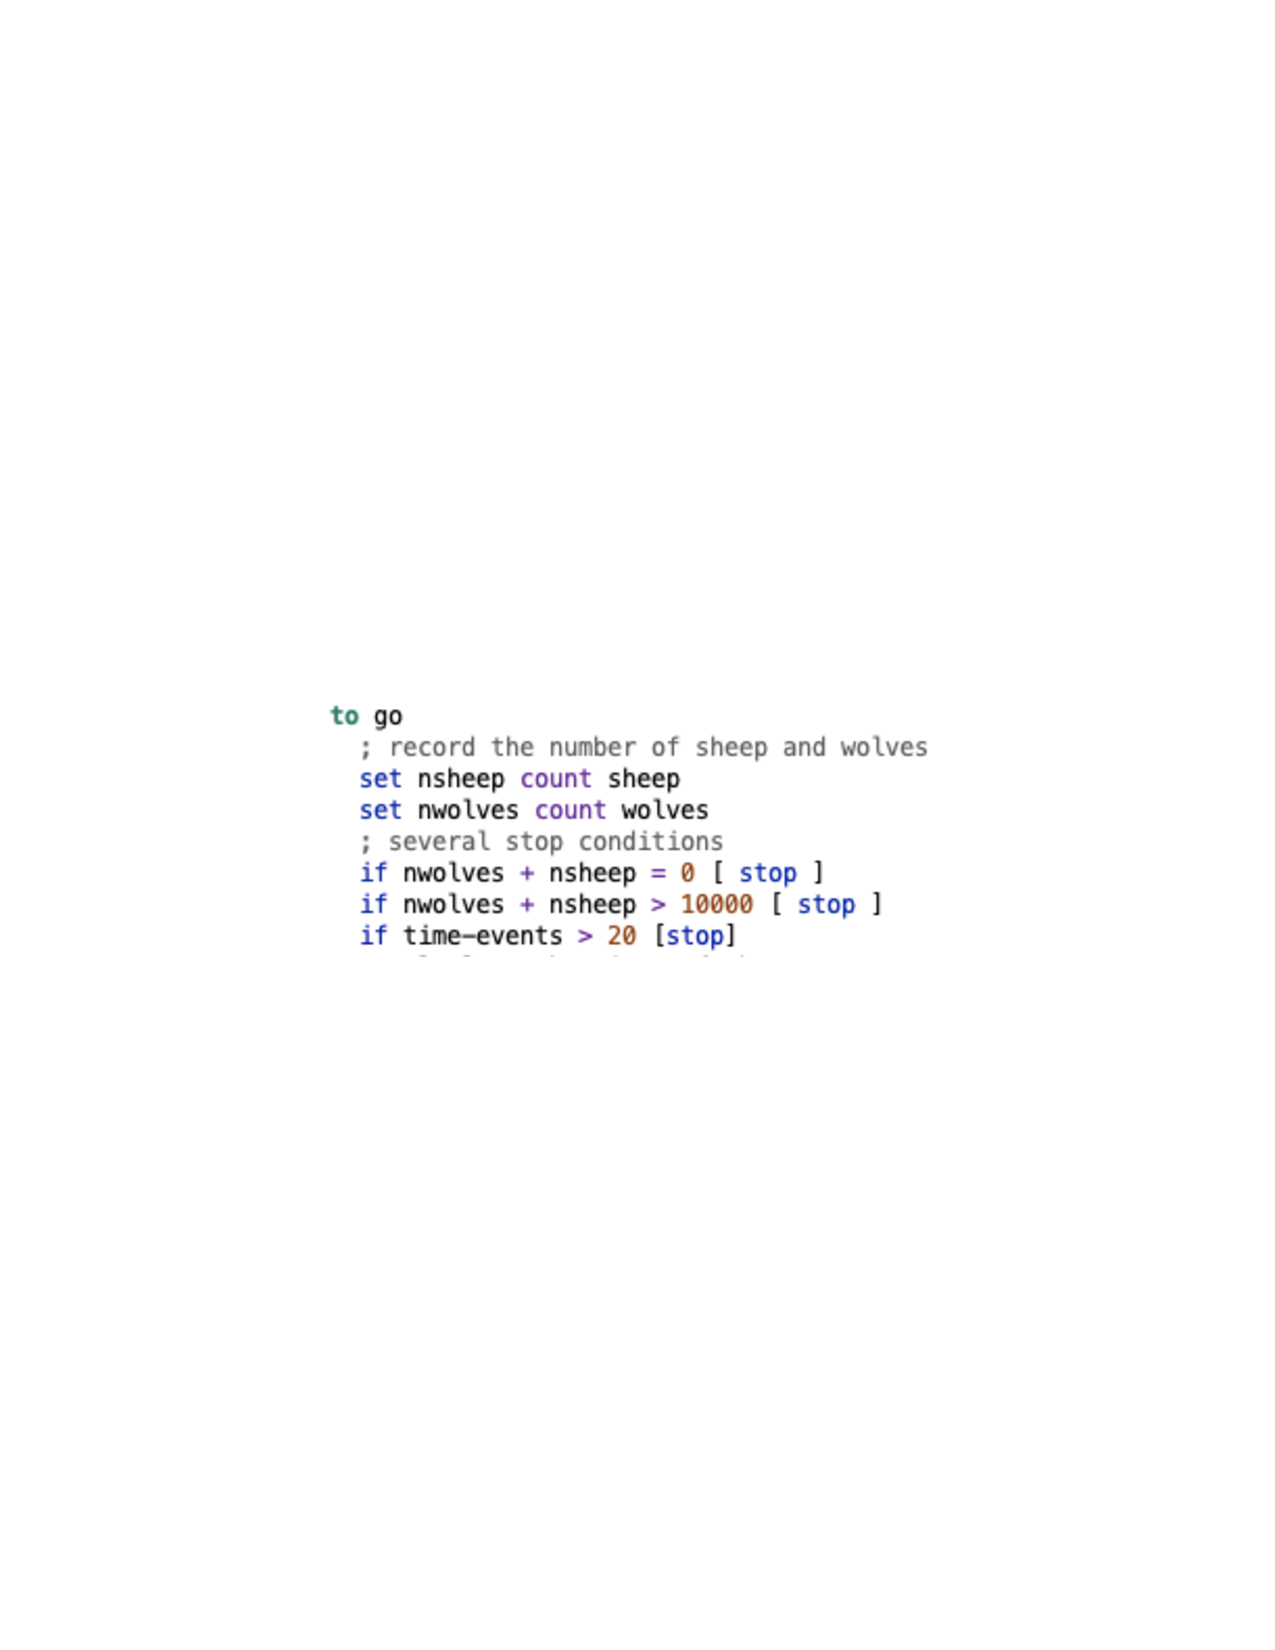
\includegraphics[height=3cm]{code1}
\end{figure}

\item To create the data that we will analyze in R, we will need to run simulations several times and export the output. To do this we select `Tools' and `BehaviorSpace'. Select `New' or `Edit' from the window that opens. You need to make 3 changes to replace the default settings (left) with the desired settings (right):

\begin{figure}
\centering
\begin{minipage}{.5\textwidth}
  \centering
  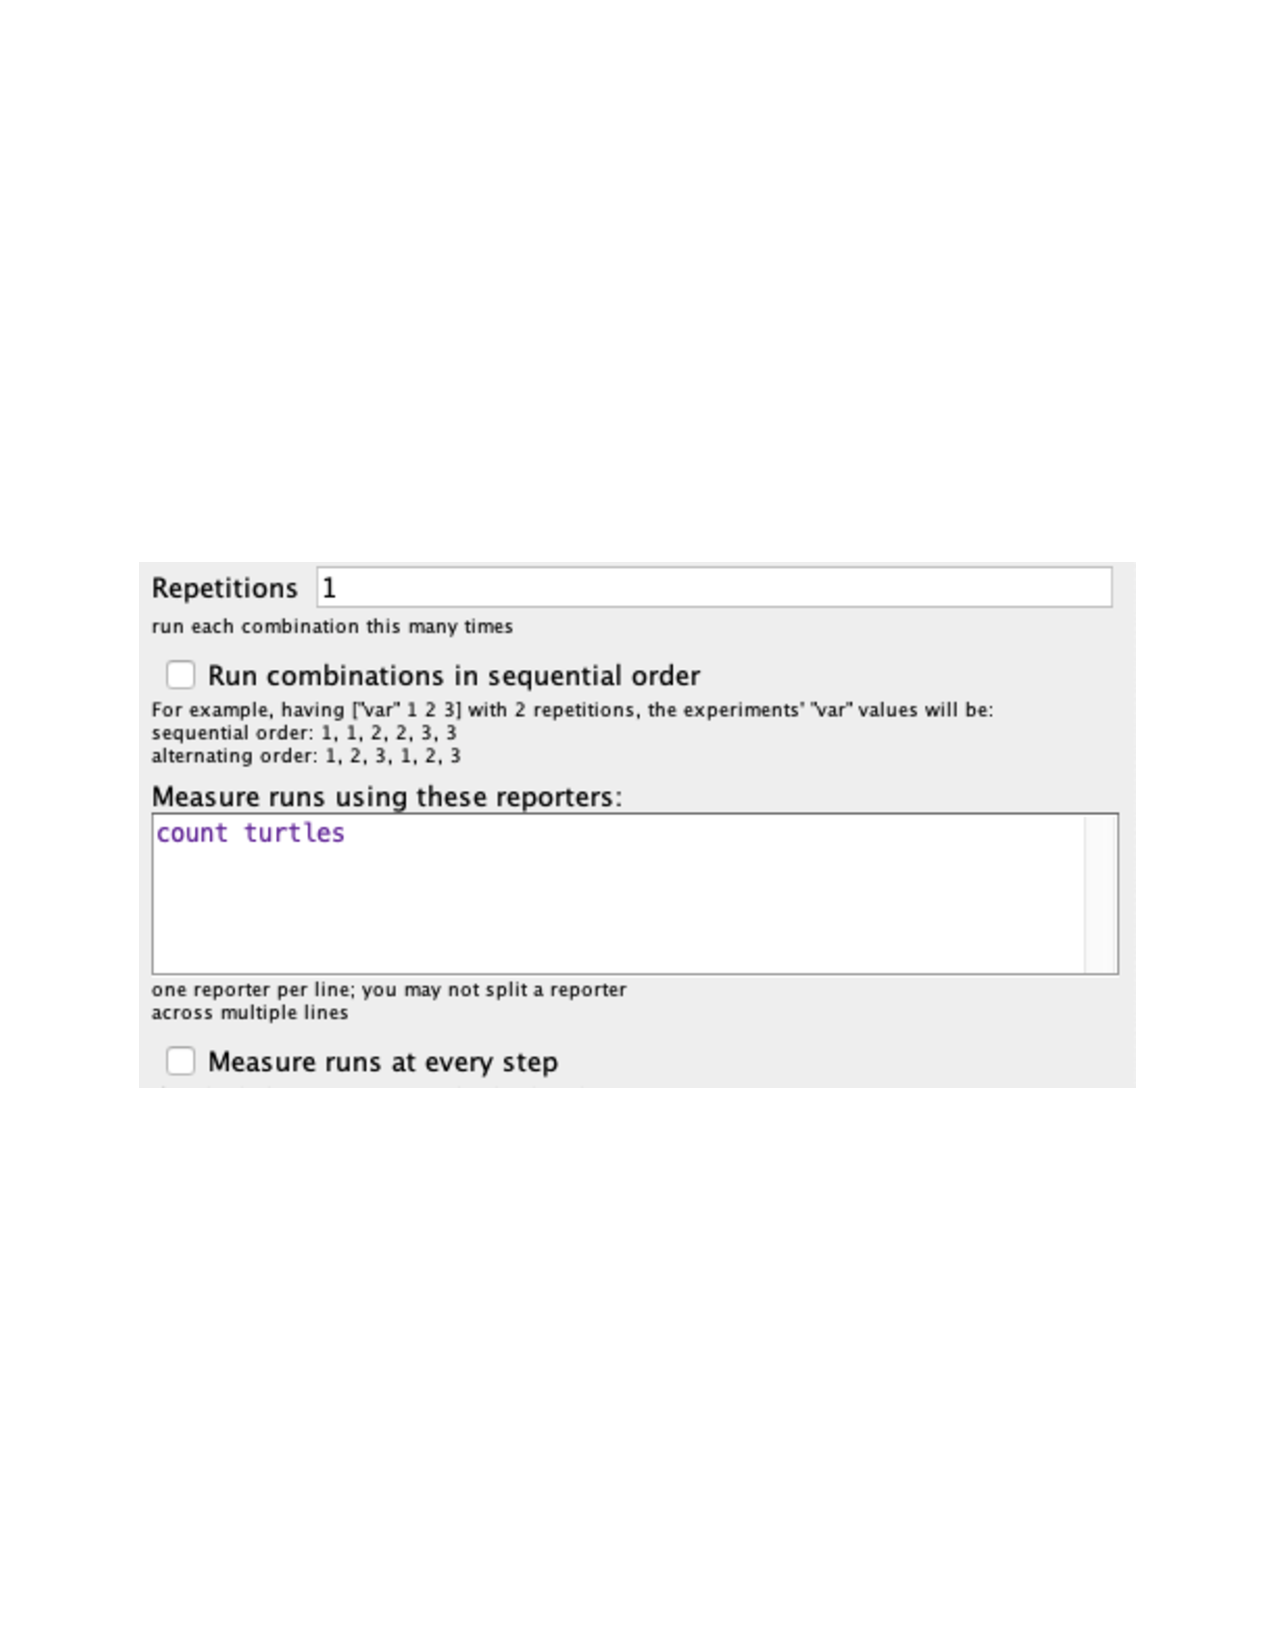
\includegraphics[width=1\linewidth]{default}
\end{minipage}%
\begin{minipage}{.5\textwidth}
  \centering
  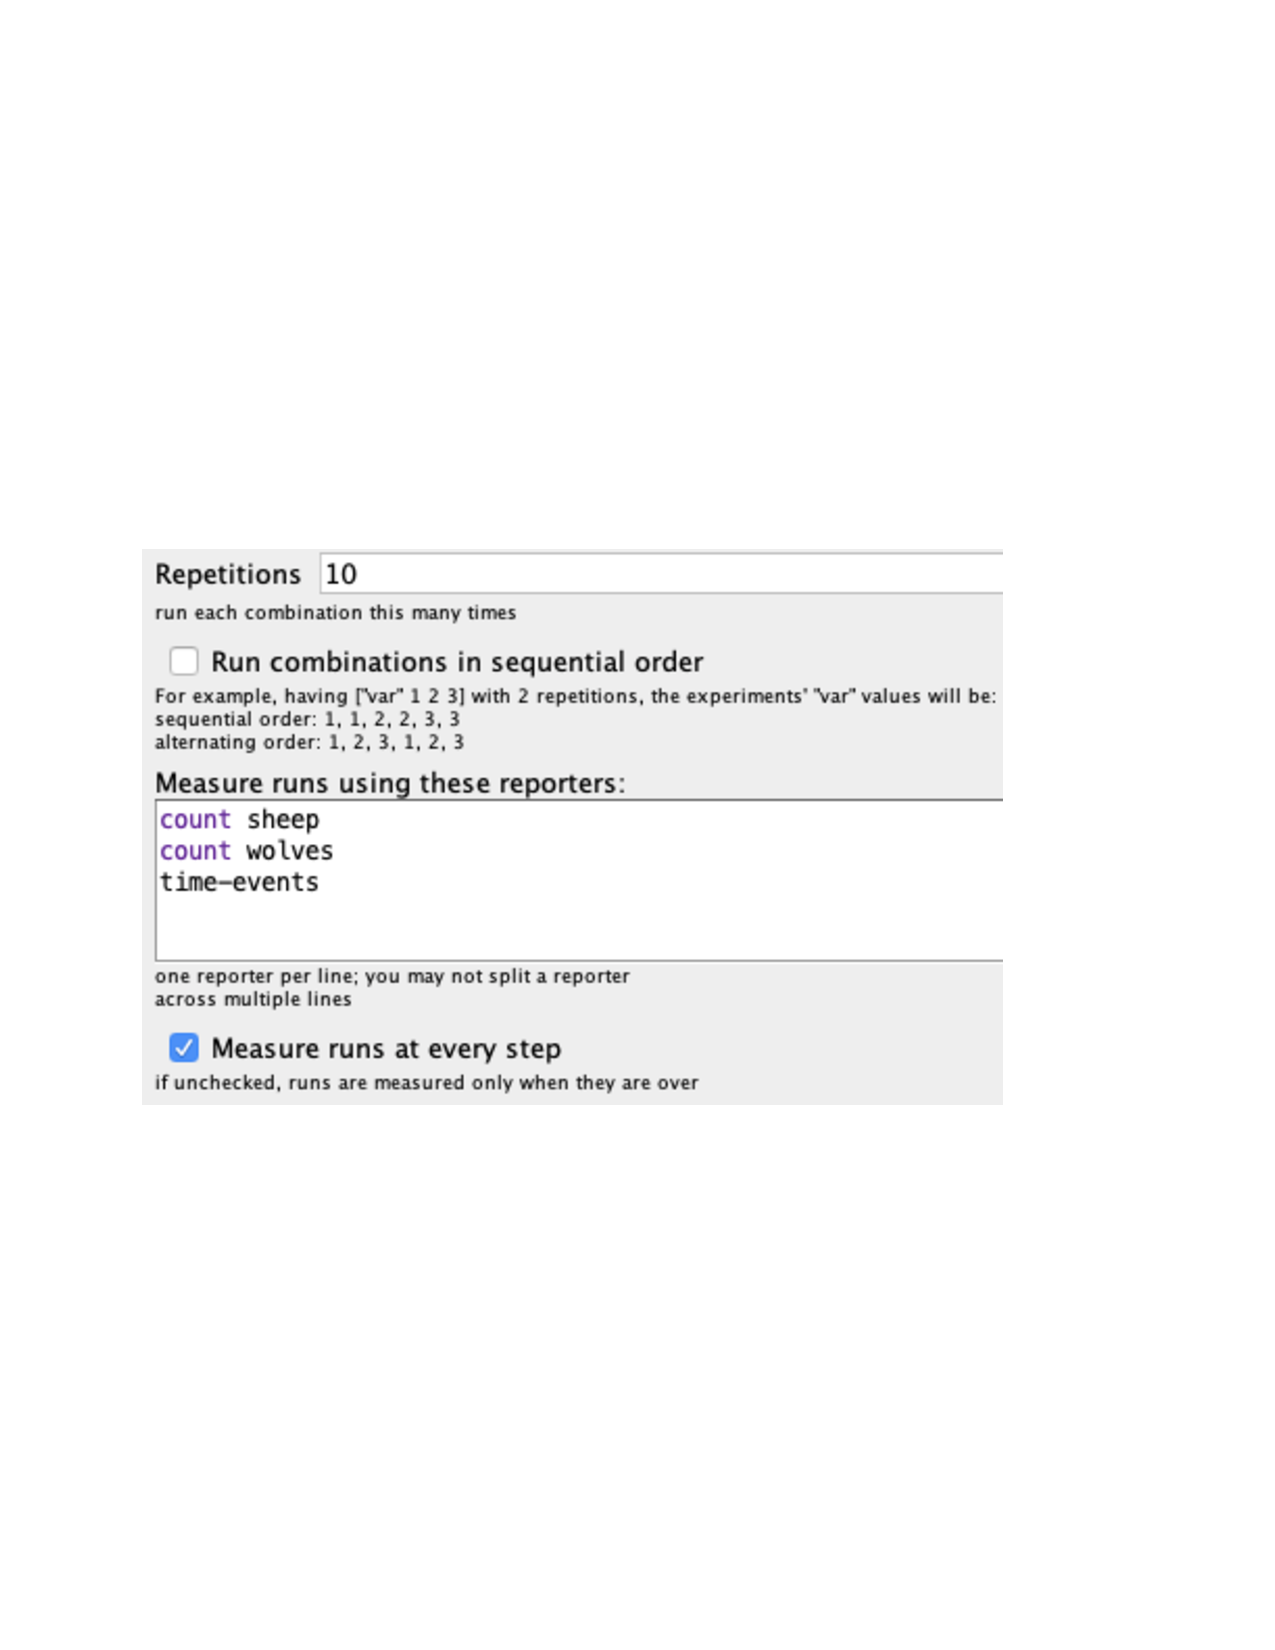
\includegraphics[width=1\linewidth]{changed}
\end{minipage}
\end{figure}
\FloatBarrier
\item Click `Ok' and `Run'. Then answer the following dialog boxes as follows:

\begin{figure}[th!]
\centering
\begin{minipage}{.5\textwidth}
  \centering
  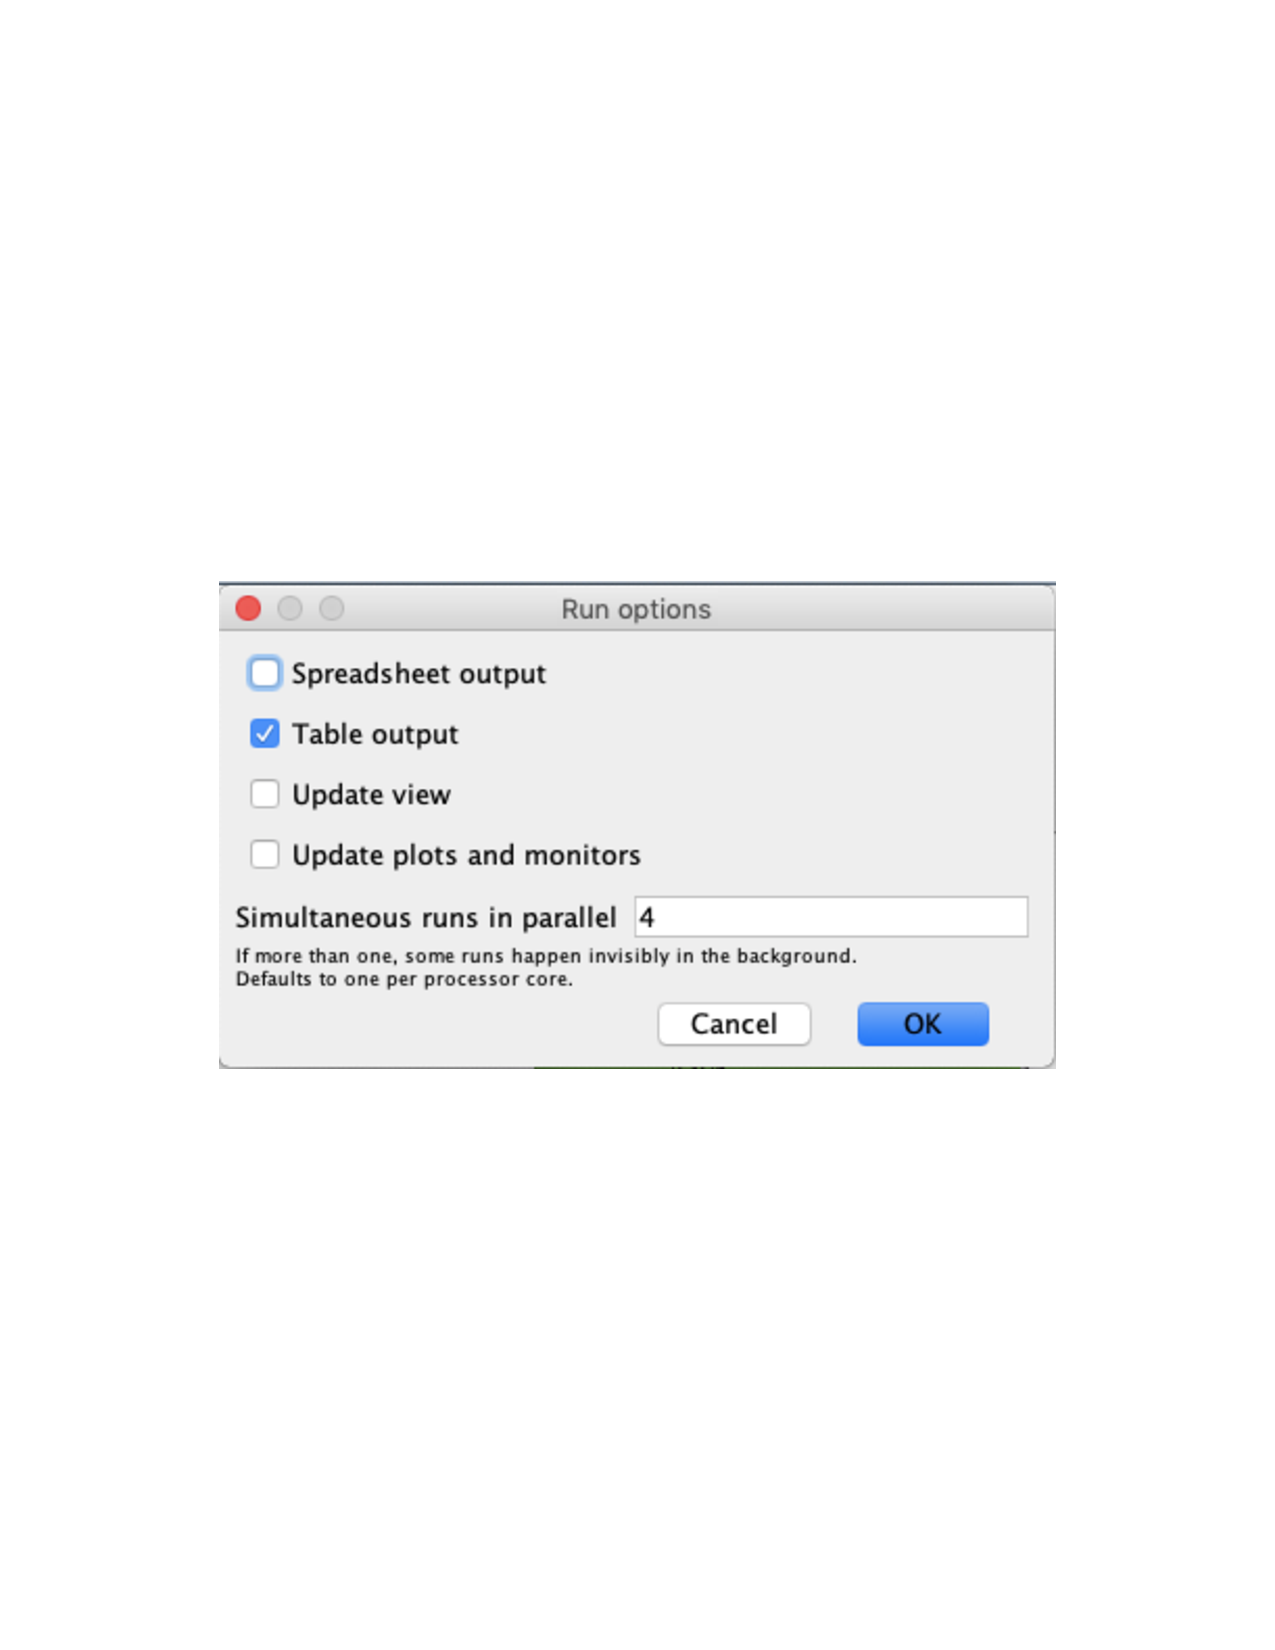
\includegraphics[width=.8\linewidth]{table}
  \label{fig:test1}
\end{minipage}%
\begin{minipage}{.5\textwidth}
  \centering
  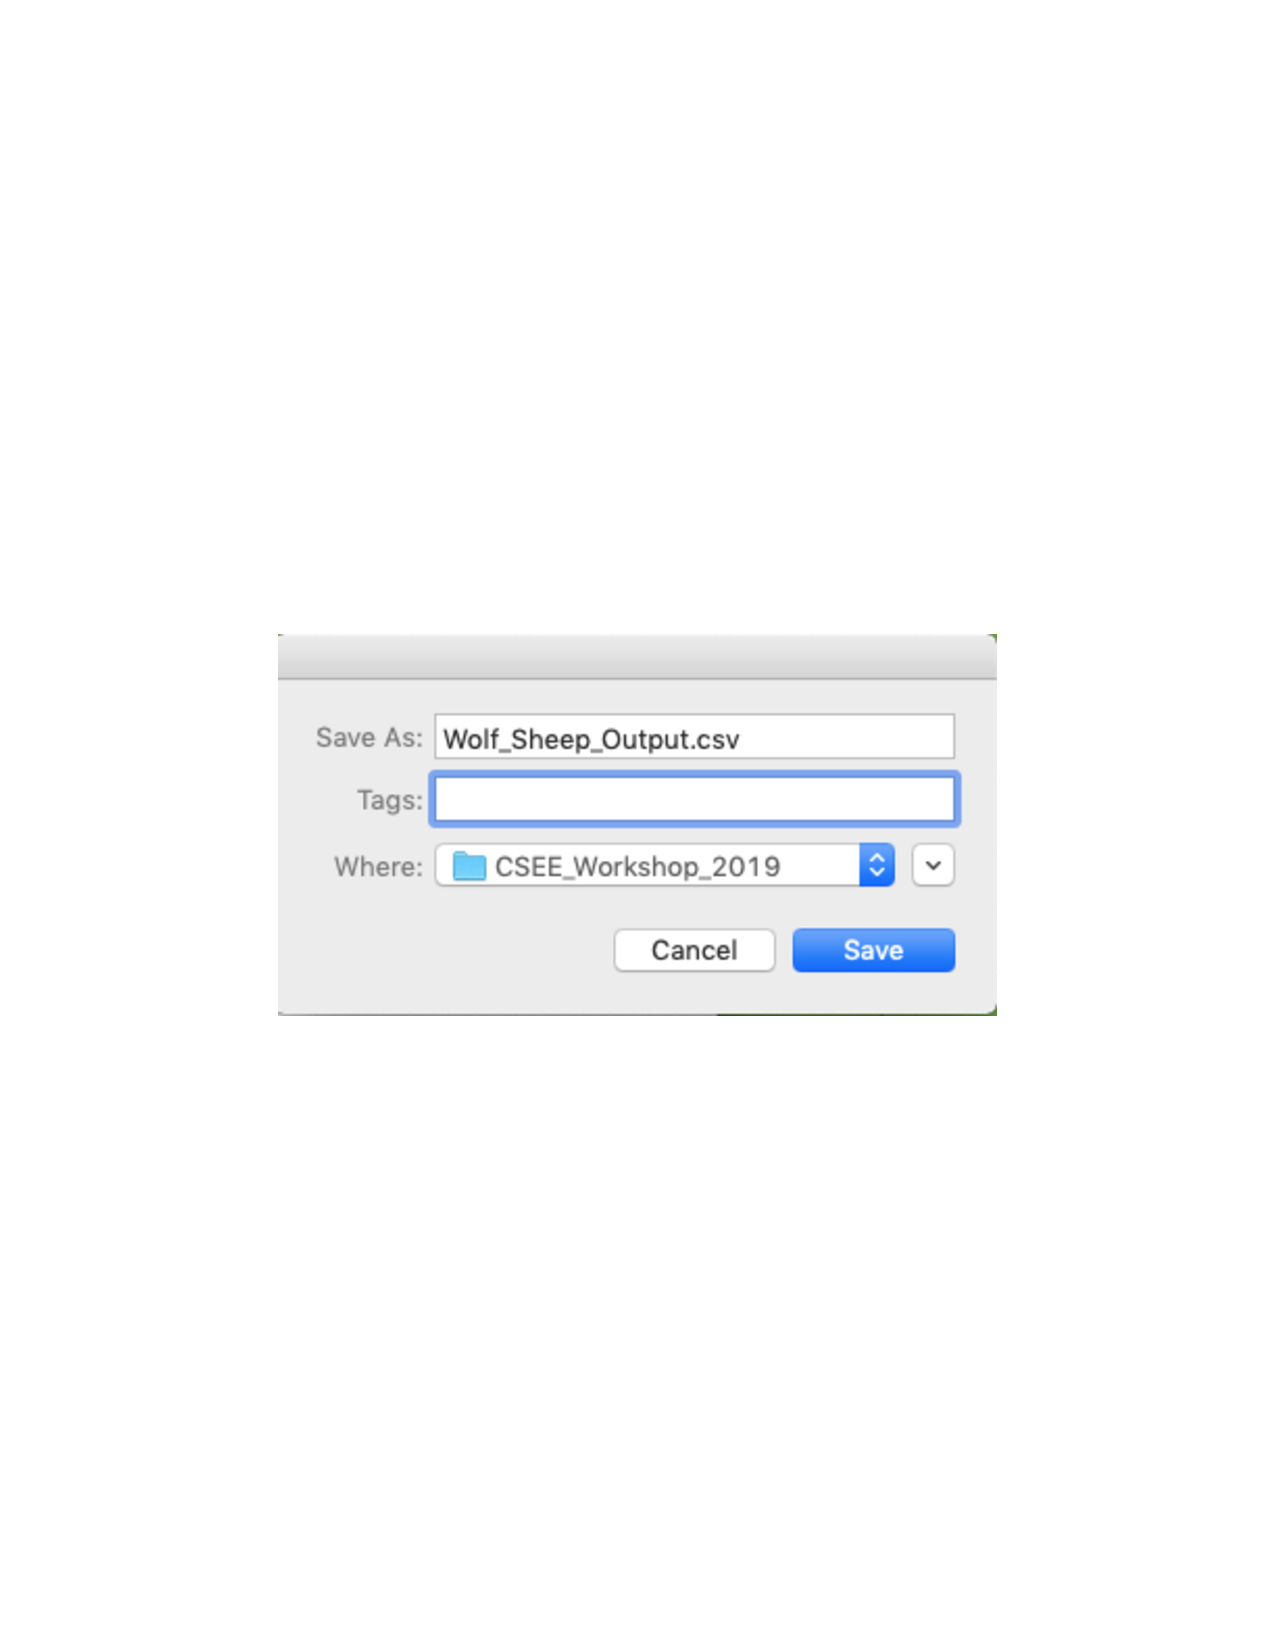
\includegraphics[width=.7\linewidth]{save}
  \label{fig:test2}
\end{minipage}
\end{figure}
\FloatBarrier
\item Now you can run your R script: \texttt{Wolf\underline{ }Sheep\underline{ }Analysis.R} (as long as you correctly set the path to find the output file). The output of the R script should resemble Figure \ref{fig:R}.
\begin{figure}[!ht]
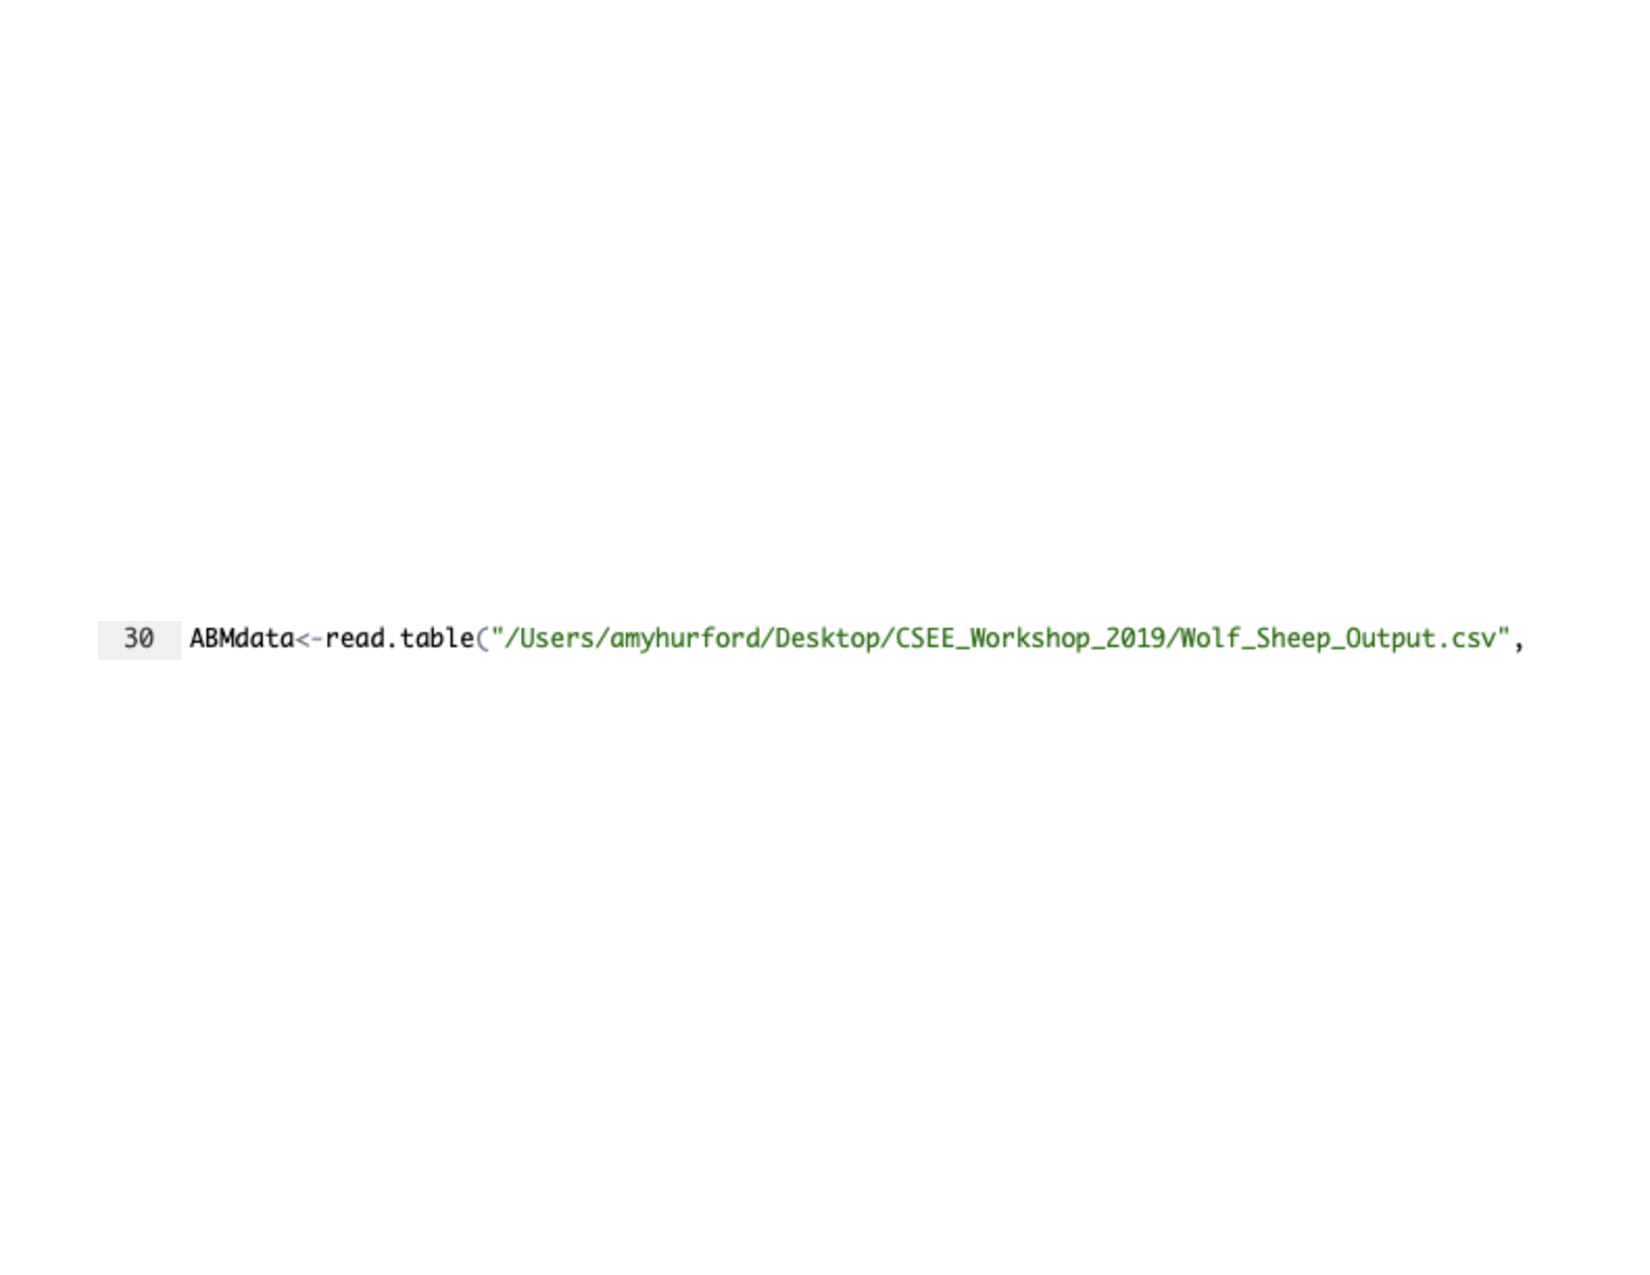
\includegraphics[height=.5cm]{path}
\end{figure}
\FloatBarrier

\item In the R script, you can set \texttt{ABM\underline{ }plot = 0} to bypass the parts of the code that visualize the results of the ABM. Change the parameter values for equations \ref{eq:PP1} and \ref{eq:PP2} and note how quickly the results via numerical integration are generated. Compare this to the time taken to simulation the ABM (in \texttt{NetLogo}) for different parameter values.

\begin{figure}[!ht]
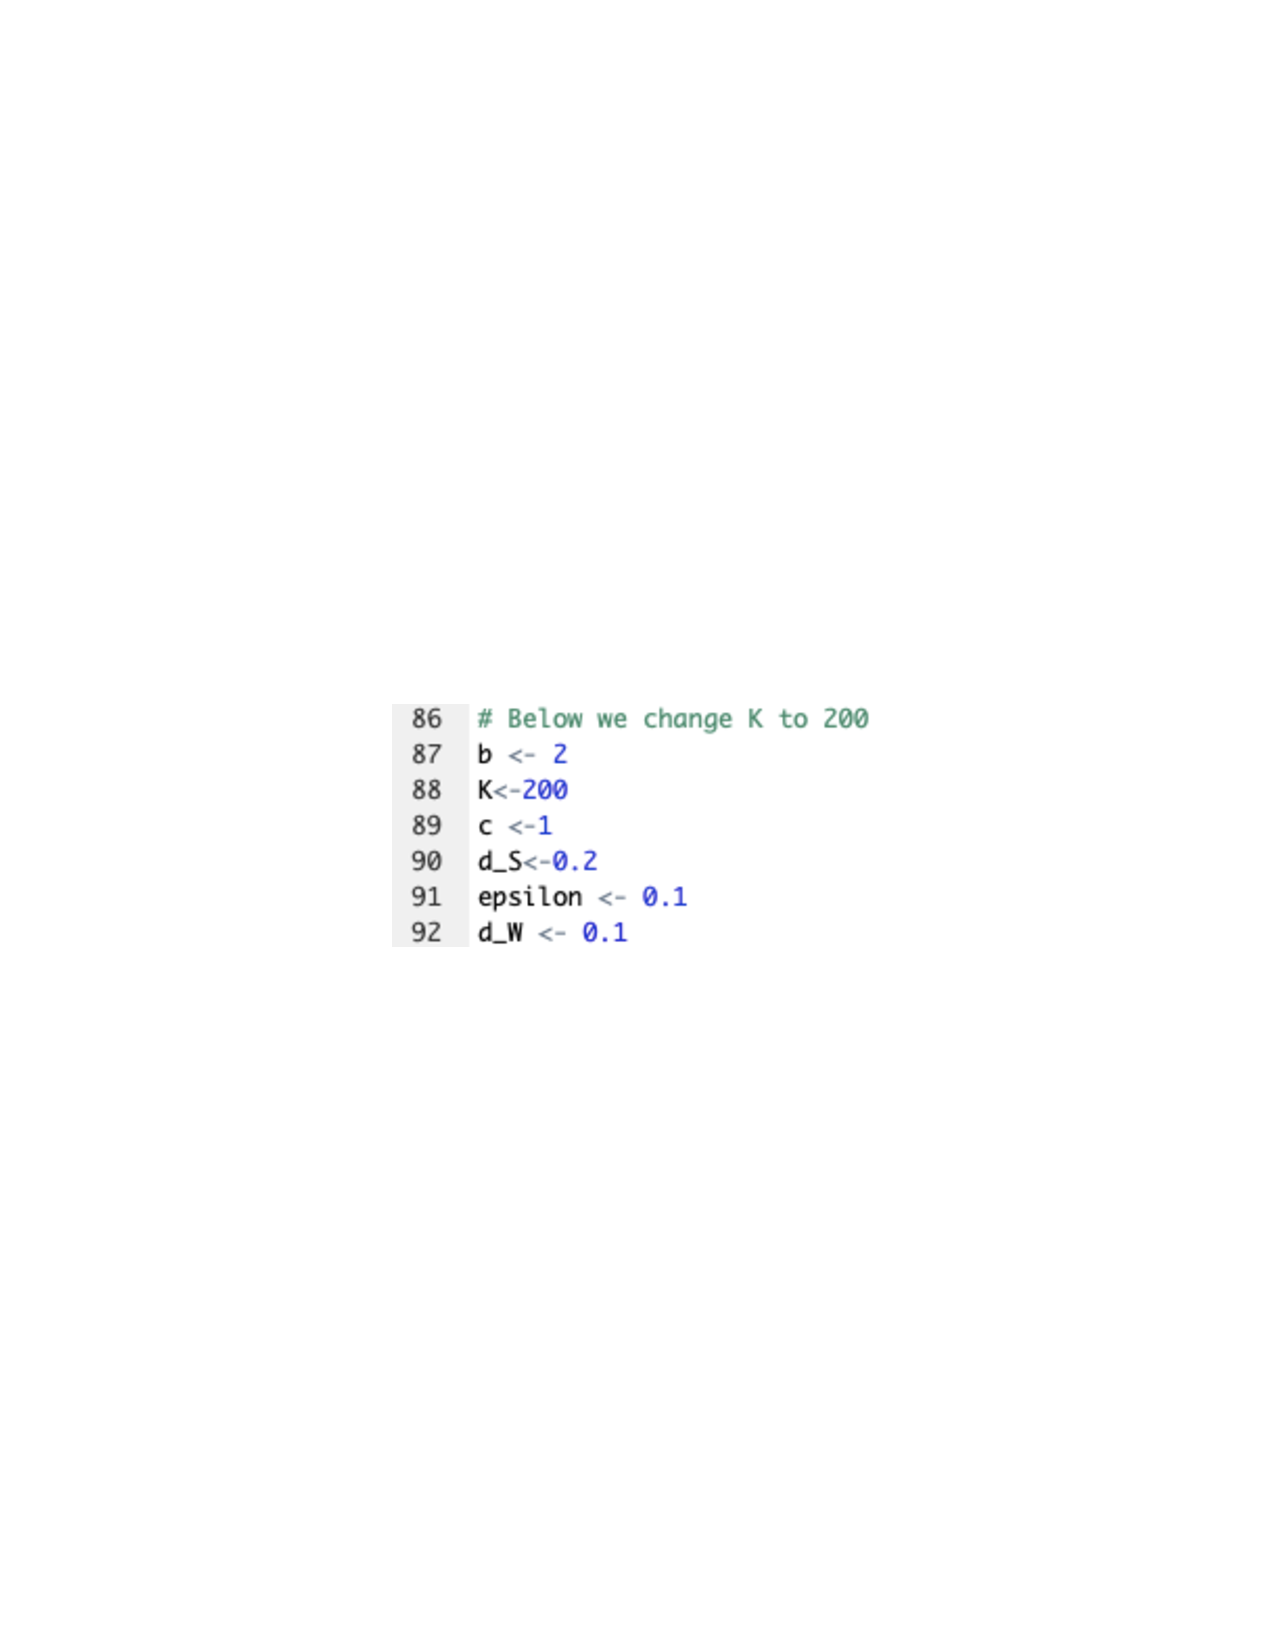
\includegraphics[height=3cm]{parameters2}
\end{figure}
\FloatBarrier

\item Try steps 3 - 8 for different parameter values.

\end{enumerate}

\begin{figure}[!ht]
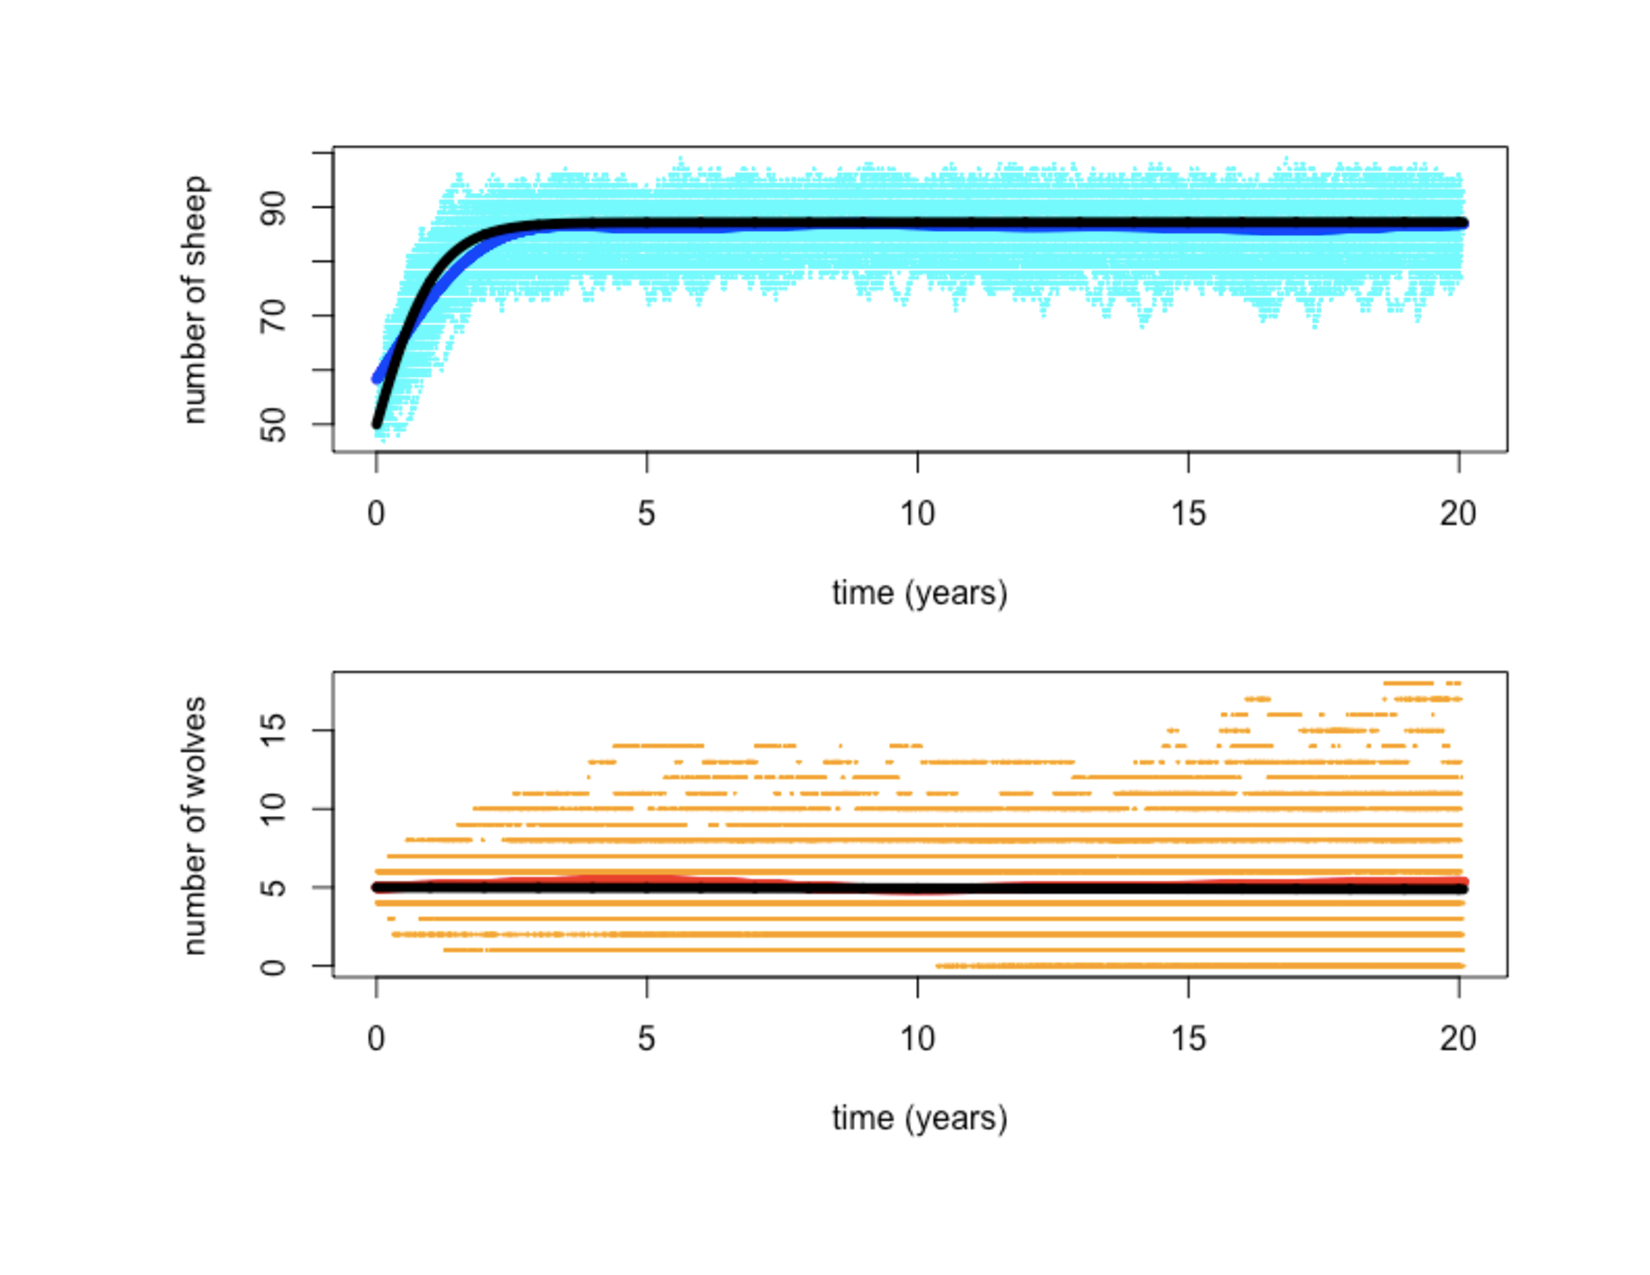
\includegraphics[height=10cm]{R_Analysis}
\caption[]{One hundred realizations of the ABM, where each realization is continued for 20 years and recording the the number of sheep (blue dots) and wolves (orange dots), with a spline fit shown as the red and blue lines. The solution to the equations \ref{eq:PP1} and \ref{eq:PP2} is the black solid line.}\label{fig:R}
\end{figure}
\FloatBarrier

This example was selected, in part, because the mean of the ABM converges quickly to the numerical solutions of the ordinary differential equations \ref{eq:PP1} and \ref{eq:PP2}. A similar example, but using the Lotka-Volterra predator-prey equations (exponential prey birth rate and a type I functional response) converged less well.

In addition to gains in computational time, an advantage of working with equations \ref{eq:PP1} and \ref{eq:PP2} is that analyses, such as those described at \cite{wiki}, provide insight into parameter regions where stable equilibrium or cyclic dynamics occur.

The \texttt{GillespieSSA} package for \texttt{R} provides many tools to perform Gillespie SSA simulations. For an example using this package to simulate the Wolf-Sheep model described by equations \ref{eq:PP1}-\ref{eq:PP2}, see the files \texttt{Rosenzweig-MacArthurSSA.R} and \texttt{RosMac2019-08-13.R}.

\section{An ABM with local infection and reproduction on a lattice}\label{sec:PA}
\subsection{A spatially explicit model}
The previous example showed us that the mean of multiple realizations of a stochastic non-spatial ABM with discrete individuals implemented following the Gillespie algorithm can be approximated by the numerical solutions of an ordinary differential equation that represents the density of wolves and sheep as a continuous quantity. In this next example, we consider discrete sites spaced at regular intervals (a lattice). The model makes the following assumptions:

\begin{description} 
\item[$\bullet$] The number of sites surrounding a focal site is $z$, i.e. $z=2$ for one dimensional space and $z=4$ for two dimensional space.
\item[$\bullet$] Sites are either unoccupied, $0$, or occupied by individuals susceptible, $S$, or infected, $I$ with a disease.
\item[$\bullet$] The infections dynamics are SI: infected individuals never recover.
\item[$\bullet$] Local transmission occurs when the infection is transmitted to a susceptible individual from an infected nearest neighbour.
\item[$\bullet$] Only susceptible individuals reproduce, reproduction can only occur if there is an unoccupied neighbouring site, and the offspring then occupies a neighbouring site. Offspring are born susceptible.
\item[$\bullet$] The model does not explicitly describe movement.
\end{description}

The events that can occur are:
\begin{description} 
\item[] \underline{Events for Susceptibles:}
\item[$E_1:$] Natural mortality: Each susceptible dies of natural cases at an average per capita rate of $d$ deaths per year. 
\item[$E_2:$] Reproduction: Each susceptible occupying a site with an adjacent empty site produces one offspring at a rate $r$ per year.
\item[$E_3:$] Local infection: Each susceptible individual, becomes infected from an infected neighbour at a rate $\beta$.
\item[] \underline{Events for Infecteds:}
\item[$E_1:$] Each infected dies of natural cases at an average rate of $d$ deaths per year. 
\item[$E_2$] Each infected dies of disease-induced mortality at a rate of $\alpha$ deaths per year.
\end{description}

The ABM is coded in \texttt{Netlogo} following the Gillespie algorithm but with slight modifications to the definition of $\mu_i$, the event that occurs on the $i^{th}$ iteration of the code. Unlike the previous example (Section \ref{sec:SSA}), where rates were equal for all prey (and all predators), for this model the neighbours of a focal individual will also affect the rates of the events. Let,

\begin{description} 
\item[$\bullet$] $c_{j,m}$ be the rate that event $E_j$ occurs for an individual indexed as $m$, 
\item[$\bullet$] $b_m = \sum_j c_{j,m}$ be sum of all the rates for the individual $m$, and redefine
\item[$\bullet$] $a_0 = \sum_m b_m$ as the sum of all the rates across all individuals.
\end{description}

For the spatially explicit ABM, we use an alternative version of equation \ref{eq:mui} whereby on the $i^{th}$ iteration of the code we: (1) randomly select an individual, $l_i$, such that,
%
\begin{equation}\label{eq:mui2}
l=l_i = \min_k\sum_{m=1}^{k} b_{m}> a_0 r_{2,i} \qquad \mbox{where $r_{2,i} \sim U[0,1]$,}
\end{equation}
%
where the probability of selecting any individual is proportional to the sum of their rates; and then (2) for the randomly selected individual, $l$, we randomly select an event,
%
\begin{equation}\label{eq:mui3}
\mu_i = \min_k\sum_{j=1}^{k} c_{j,l}> b_l r_{3,i} \qquad \mbox{where $r_{3,i} \sim U[0,1]$.}
\end{equation}
%
The time to the next event, $\tau_i$, is calculated using equation (\ref{eq:taui}), but where $a_0$ is as defined above in this section as the third bullet point. We calculated $\mu_i$ using this two-step process to take advantage of \texttt{NetLogo}'s strength in cataloguing individual-level (\texttt{turtles-own}) properties, which were used to evaluate \ref{eq:mui2}. If this same calculation were performed in \texttt{MATLAB} or \texttt{R}, which have more functions available to work with vectors, we might have implemented equations \ref{eq:mui2} and \ref{eq:mui3} differently.

\subsection{The pair approximation equations}
For our spatially explicit disease model, we will derive a system of ordinary differential equations describing the change in the proportion of site pairs, $p_{\sigma \sigma'}$, where $\sigma$ and $\sigma'$ are sites that are either empty, $0$, or occupied by individuals that are susceptible, $S$, or infected, $I$. The equations are derived in \cite{sato}, but we opt for the notation of \cite{boots}, which we find more accessible (note that we set $P = 0$ in equations 1-6 of \cite{boots} because we assume only local transmission for our models). The rate of change in the proportion of sites that are a particular type of pair depends on the status of the neighbouring sites. We use $q_{\sigma / \sigma' \sigma''}$ to denote the probability that a neighbouring site is type $\sigma$ for a pair of sites ($\sigma'$ and $\sigma''$). The / notation in $q_{\sigma / \sigma' \sigma''}$ indicates a conditional probability, where the fixed condition is the type of paired site. For a two-dimensional lattice, any particular site will have four neighbours, $z=4$, and $\theta = 1/z$ is the proportion of nearest neighbour sites that are any one site. The dynamics of the change in the proportion of each type of paired sites in the landscape is described by the equations:
%
\begin{eqnarray}
\frac{dp_{SS}}{dt} & = & 2r(\theta + (1-\theta)q_{S/0S})p_{S0} - (2d + 2\beta(1-\theta)q_{I/SS})p_{SS},\label{eq:pSS}\\
\frac{dp_{S0}}{dt} & = & r(1 - \theta)q_{S/00}p_{00} + dp_{SS} + (d+\alpha)p_{IS} - (d +r(\theta + (1-\theta)q_{S/0S})+\beta q_{I/0S})p_{S0},\label{eq:pS0}\\
\frac{dp_{00}}{dt} & = & 2p_{S0} + 2(d+\alpha)p_{I0} - 2r(1-\theta)q_{S/00}p_{00},\\
\frac{dp_{II}}{dt}& = & 2\beta(\theta + (1-\theta)q_{I/IS})p_{IS} - 2(d+\alpha)p_{II},\\
\frac{dp_{IS}}{dt}& = & r(1-\theta)q_{S/0I}p_{I0} + \beta q_{I/SS}p_{SS} - (2 d + \alpha + \beta(\theta + (1-\theta)q_{I/SI}))p_{IS},\\
\frac{dp_{I0}}{dt} & = & \beta (1 - \theta)q_{I/S0}p_{S0} + dp_{IS} + (d + \alpha)p_{II} - (d + \alpha+r(1-\theta)q_{S/0I})p_{I0},\label{eq:pI0}
\end{eqnarray}
%
\cite{sato, boots}. We note that the order of site types does not matter, such that the change in paired sites $S0$ and $0S$ are represented by equation \ref{eq:pS0}, and the same is true of the other combinations of different site pairs: the ordering does not matter.

To understand equations \ref{eq:pSS}-\ref{eq:pI0}, we will step through each term in equation \ref{eq:pSS}, which describes the change in the proportion of paired sites that are both occupied by susceptible individuals. First, we note that an $SS$ paired site is created from an $S0$ site, where reproduction occurs into the $0$ site. The proportion of sites that are $S0$ is $p_{S0}$, and there are two possible orderings for this site type: $S0$ or $0S$. For these $S0$ paired sites, one of the nearest neighbours of the $0$ site is the $S$ site that comprises the other half of the pair, which is the fraction $\theta$ of all the neighbours. To calculate the status of the other $z-1$ neighbours, we note that $q_{S/0S}$ is the probability that an $0S$ paired site has an $S$ neighbour. The reproductive rate is $r$, and so the first term of the equation \ref{eq:pSS} describes the rate that new $SS$ sites are created from $S0$ sites through reproduction. The model assumes that in some small increment of time only one change can happen, and so it is not possible that a $00$ paired site can change to an $SS$ paired site without first becoming an $S0$ paired site.

The last term in equation \ref{eq:pSS} describes the rate of loss of $SS$ paired sites to $S0$ or $SI$ sites. Natural mortality occurs at a rate $d$, and the rate that natural mortality occurs on either of the two $SS$ sites is $2d$. In addition, infection may occur on either of the two sites at rate $\beta$, if a neighbouring site is $I$. Since the pair is $SS$, we know that each $S$ site has 1 nearest neighbour that is not $I$. The fraction of remaining nearest neighbours is $1-\theta$, and the probability that one of these neighbours is infected, is $q_{I/SS}$. The remaining equations (\ref{eq:pS0}-\ref{eq:pI0}) can be interpreted similarly by considering the processes that create or destroy particular site pairs.

The frequency of each site type in the landscape is calculated as the sum,
%
\begin{equation}\label{eq:psigma}
p_\sigma' = \sum_{\sigma\in\{0,S,I\}} p_{\sigma \sigma'}.
\end{equation}

Note that $SS$ site pairs do not contribute twice as many $S$ individuals to the population as $S0$ patches because there are two ways to make a $S0$ pair: either $S0$ or $0S$.

\subsection{Closing the pair equations}
The challenging aspect of equations \ref{eq:pSS}-\ref{eq:pI0} is that the probabilities for the neighbouring sites of a pair, $q_{\sigma / \sigma' \sigma''}$, can only be accurately calculated if the proportion of specific site triples are known, which in turn, can only be accurately calculated if the proportion of site quadruples is known, and so forth. While we could derive equations for the changes in the number of site triples, or even higher combinations of site pairings, our goal is to approximate the ABM, rather than to create an alternative version of a complex model. The process of ending the infinite dependency of site combination changes on higher order site combinations through approximation is referred to as `closure'. The R script that we provide considers three types of closure: (1) the ordinary pair approximation (OPA), (2) the improved pair approximation (IPA, \cite{sato}), which may be more accurate for the specific SI disease model that we are studying, and 3) the Singlet Density Approximation (SDA; \cite{matsuda}).

\subsubsection{Ordinary Pair Approximation}
The OPA assumes that $q_{\sigma / \sigma' \sigma''} \approx q_{\sigma / \sigma'}$, which means that the approximation assumes that the status of the other patch, $\sigma''$, does not affect the types of neighbours that surround the focal patch. The formula for conditional probabilities states that,

\[
q_{\sigma / \sigma'} = \frac{p_{\sigma \sigma'}}{p_{\sigma'}}
\]
where $p_{\sigma \sigma'}$ for all possible $\sigma \sigma'$ combinations can be calculated by numerically integrating equations \ref{eq:pSS}-\ref{eq:pI0} where $p_{\sigma'}$ is the proportion of sites that are of type $\sigma'$, which is determined by summing proportion of all site pairs that have at least one site of the type $\sigma'$. The notation $p_{\sigma \sigma'}$ does not attach any significance attached to the site type appearing in the first or second subscript position. Therefore, the OPA could equivalently be calculated as $q_{\sigma / \sigma' \sigma''} \approx q_{\sigma / \sigma'}$ or $\approx q_{\sigma / \sigma''}$.

\subsubsection{Improved Pair Approximation}
The IPA notes that similar types of sites tend to aggregate in space. Such that where $0 \leq \epsilon \leq 1$,
%
\begin{equation}
q_{S/00} = \epsilon q_{S/0}, \label{eq:IPA1}
\end{equation}
%
since the combination of two empty sites is less likely to have a neighbour that is $S$, than just one empty site whose other partner might well be $S$. Furthermore, the IPA assumes,
%
\begin{equation}
q_{I/S\sigma}  \approx q_{I/S}\qquad \mbox{and} \qquad q_{S/0I} \approx q_{S/0}, \label{eq:IPA2}
\end{equation}
%
which are OPA-type approximations. Finally, equations \ref{eq:IPA1} and \ref{eq:IPA2} and the identity relationship for conditional probabilities, then implies that,
%
\begin{equation}
q_{S/0S} = 1 - q_{I/0} - \epsilon q_{0/0}\label{eq:IPA3}
\end{equation}
%
and no other approximations are needed since other possible $q_{\sigma/\sigma'\sigma''}$ do not appear in equations \ref{eq:pSS}-\ref{eq:pI0}. \cite{sato} estimates that for a two-dimensional lattice ($z=4$), that $\epsilon = 0.8093$. This $\epsilon = 1$ then the IPA reduces to an OPA.

\subsubsection{Singlet Density Approximation}
The Singlet Density Approximation (SDA) approximates $q_{\sigma / \sigma' \sigma''}$ by assuming the probability that a $\sigma$ site is a neighbour of a $\sigma'\sigma''$ pair is equal to the landscape-wide frequency of $\sigma$, i.e.
%
\begin{equation}
q_{\sigma / \sigma' \sigma''} = p_\sigma,
\end{equation}
%

\subsection{Code files}
\begin{description}
\item[Local SI.nlogo] A Netlogo program that performs a Gillespie algorithm implementation of the pair approximation equations for the local infection spread model (equations \ref{eq:pSS}-\ref{eq:pI0}).
\item[Local\underline{ }SI\underline{ }Analysis.R] This \texttt{R} file numerically solves the pair equations \ref{eq:pSS}-\ref{eq:pI0} and is able to reproduce Figure 3 of \cite{sato} (see Figure \ref{fig:sato}). The file also imports the results of \texttt{Local SI.nlogo} simulations that have been saved as the files \emph{SI\underline{ }Output.csv} and \emph{SI\underline{ }Output2.csv} and compares the agreement between the ABM and the numerically solved pair equations with four different closures (Figure \ref{fig:closure}) .
\end{description}


\begin{figure}[!ht] 
\includegraphics[height=12cm]{sato3} 
\caption[]{We numerically solve equations \ref{eq:pSS}-\ref{eq:pI0} using the IPA to reproduce Figure 3 of \cite{sato}. The parameter values are $r=4$, $\alpha = 0$, $d=1$, $\epsilon = 0.8093$ and $\beta$ as described by the panel titles.} \label{fig:sato}
\end{figure}

\begin{figure}
\centering
\begin{minipage}{.5\textwidth}
  \centering
  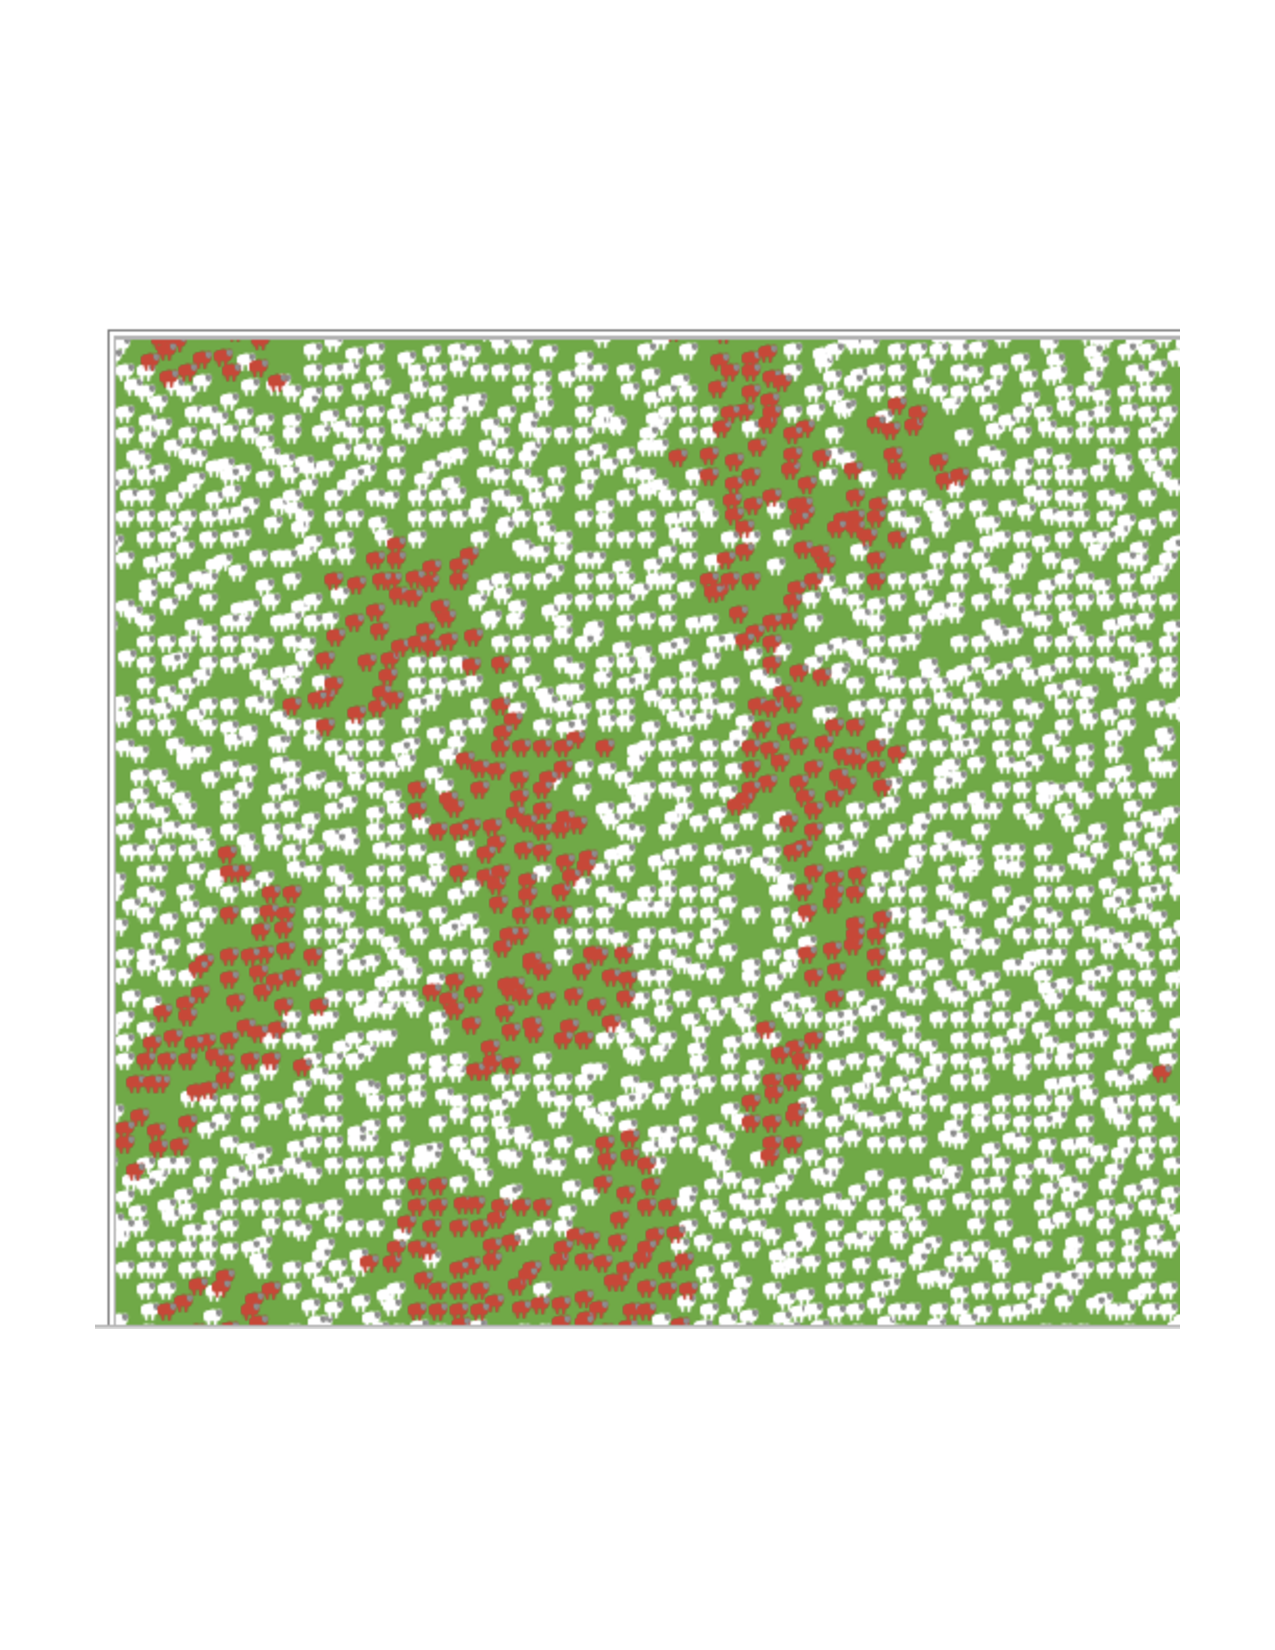
\includegraphics[width=1.1\linewidth]{NetlogoBeta4}
\end{minipage}%
\begin{minipage}{.5\textwidth}
  \centering
  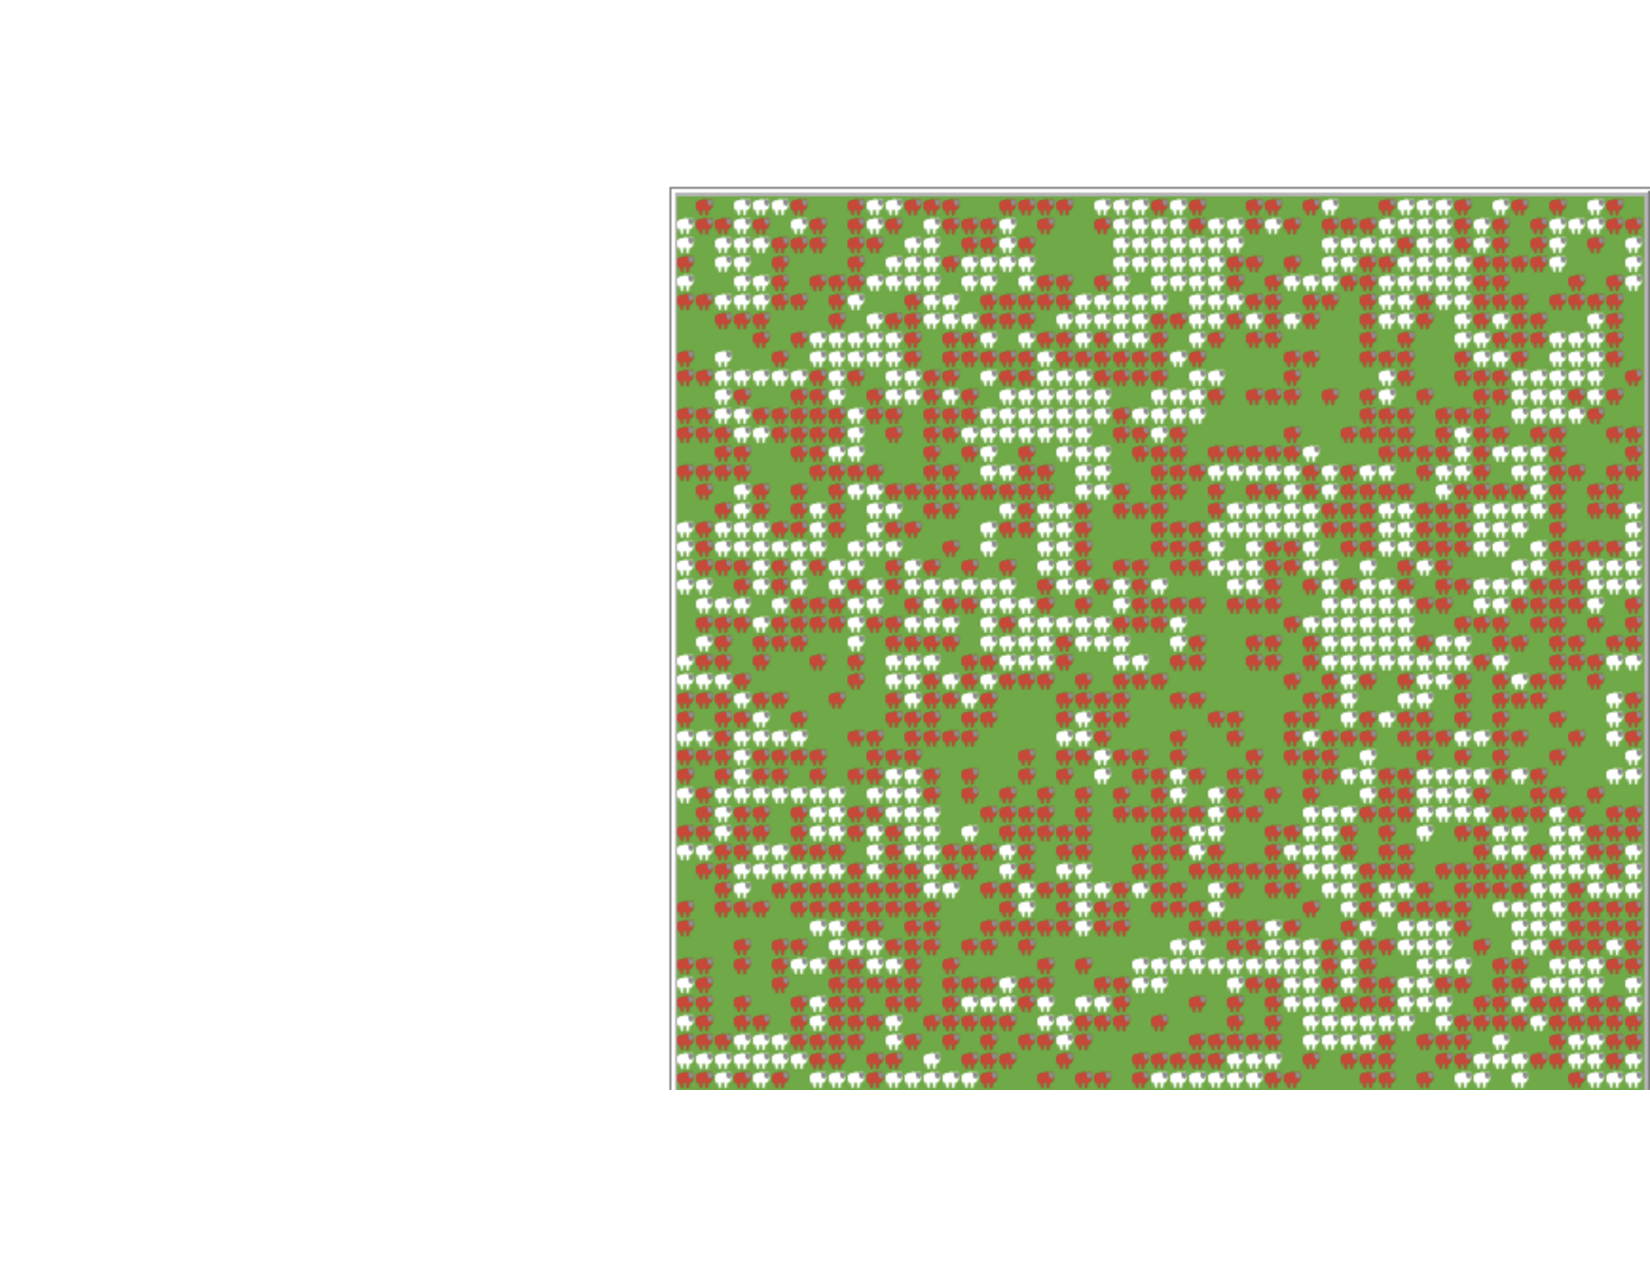
\includegraphics[width=.95\linewidth]{NetlogoBeta1}
\end{minipage}
\vspace{-2cm}
\caption[]{Simulation results generated by \texttt{Local SI.nlogo}. When the transmission rate is much higher than the natural mortality rate infections are found in clusters (left), but when the transmission rate is more similar to the natural mortality rate empty space frequently becomes available for susceptible individuals to reproduce into allowing susceptible sheep to persist in the population long term (right). For the panel on the left, $\beta = 4$, $t = 0.55$ years, and eventually all sheep become infected. For the panel on the right, $\beta = 1$ and the figure shows a dynamic steady state reached after 20 years. The other parameter values are $r=4$, $d=1$ and $\alpha=0$.}\label{fig:netlogobeta} 
\end{figure}

\begin{figure}
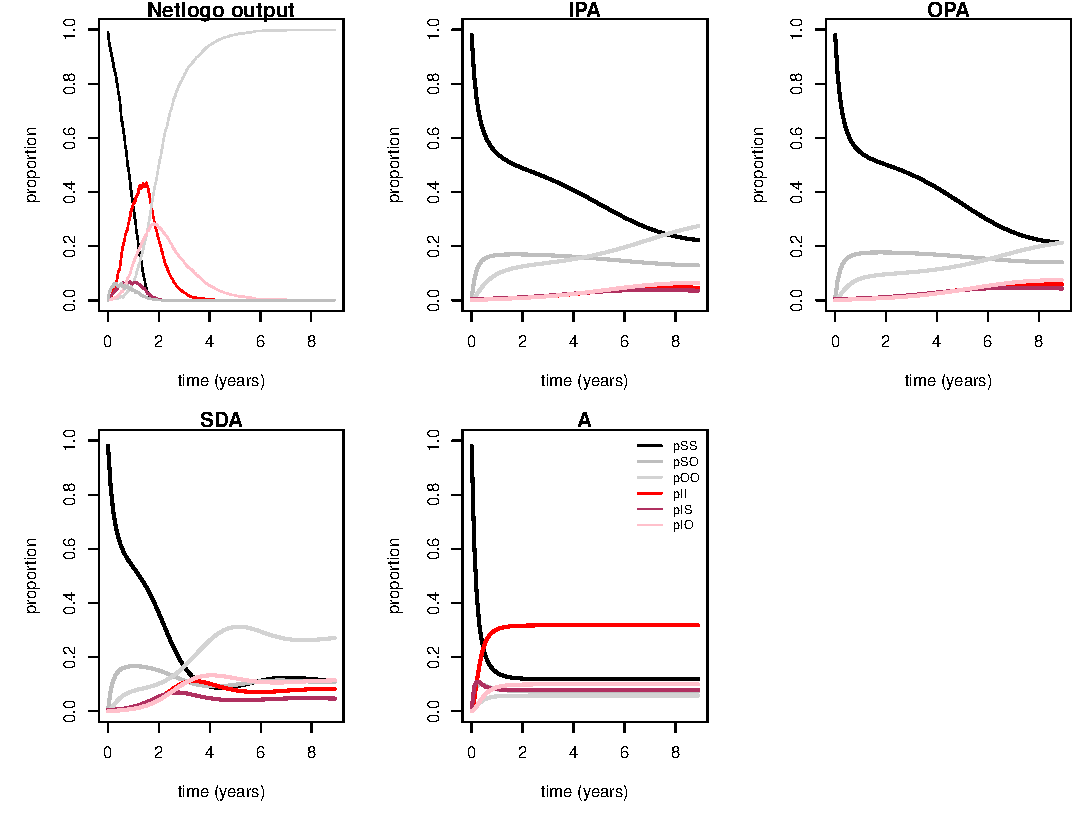
\includegraphics[width=\textwidth]{closure_comp}
\caption[]{Generated by \texttt{Local\underline{ }SI\underline{ }Analysis.R}. This figure compares the output of  \texttt{Local SI.nlogo} to the numerical solutions of the pair equations \ref{eq:pSS}-\ref{eq:pI0} using four different closures. A different closure may be needed to produce better agreement, or a system of triplet equations might be derived for better accuracy.}\label{fig:closure} 
\end{figure}
\FloatBarrier
\section{Additional reading}\label{sec:AR}

We will update this section with recommendations of required reading in a future version of this document.

\makeatletter
\renewcommand\@biblabel[1]{}
\makeatother

\begin{thebibliography}{10}

\bibitem[Boots and Sasaki, 1999]{boots} Boots, M. and A. Sasaki. 1999. `Small worlds' and the evolution of virulence: infection occurs locally and at a distance. Proc R Soc Lond B 266: 1933-1938.

\bibitem[Gillespie, 1977]{Gillespie} Gillespie, D. T. 1977. Exact Stochastic Simulation of Coupled Chemical Reactions. The Journal of Physical Chemistry 81(25): 2340-2361.

\bibitem[Matsuda et al., 1992]{matsuda} Matsuda, H., N. Ogita, A. Sasaki, and K. Sato. 1992. Statistical Mechanics of Population: The lattice lotka-volterra model. Progress of Theoretical Physical 88(6):  1035-1049.

\bibitem[Muller and Kuttler, 2015]{Muller}M\"uller, J. and C. Kuttler, 1995. Methods and Models in Mathematical Biology: Deterministic and Stochastic Approaches. Lecture Notes on Mathematical Modelling in the Life Sciences. Springer. Berlin.

\bibitem[Sato et al., 1994]{sato} Sato, K.,  H. Matsuda, A. Sasaki. 1994. Pathogen invasion and host extinction in lattice structured populations. Journal of Mathematical Biology 32: 251-268.

\bibitem[Wikipedia, 2019]{wiki} Wikipedia, 2019. Paradox of enrichment. \url{https://en.wikipedia.org/wiki/Paradox_of_enrichment}.

\end{thebibliography}
\newpage
\renewcommand\appendix{\clearpage\pagenumbering{arabic}\origappendix}
\renewcommand{\theequation}{A.\arabic{equation}}
\setcounter{equation}{0} 
\renewcommand{\thefigure}{A.\arabic{figure}}
\setcounter{figure}{0} 
\renewcommand{\thetable}{A.\arabic{table}}
\setcounter{table}{0} 
\setcounter{section}{0} 
\renewcommand{\thesection}{A.\arabic{section}}
\section{Appendix}\label{sec:Appendix}
\subsection{Software requirements}
\label{sec:software}
To complete all aspects of this workshop you will need the following software:
\begin{description}
\item[$\bullet$] \texttt{Netlogo}. See here \url{https://ccl.northwestern.edu/netlogo/download.shtml} for download information. nlogo files were written in Version 6.0.4.
\item[$\bullet$] \texttt{R}. See here \url{https://www.r-project.org/} for download information. Files are compatible with version 3.5.1 \emph{``Feather Spray''}. Some \texttt{R} files were written using \texttt{RStudio} as an interface, but \texttt{RStudio} is optional, not mandatory. The following packages need to be installed: \texttt{deSolve} and \texttt{GillespieSSA}.
\end{description}


\subsection{Background on software and package choices and installation problems}

Using a Macbook Air (2015) operating on Mojave macOS 10.14.6, I began working on these workshop materials by searching for an R package to simulate an ABM. I package I found was \texttt{RNetLogo}. This package is dependent on a \texttt{NetLogo}, so I updated to the most recent NetLogo (6.0.4). I had problems with this install, but eventually I found this solution \cite{soln}. Specifically, I opened a terminal window and typed the command as described here:

\begin{figure}[!ht]
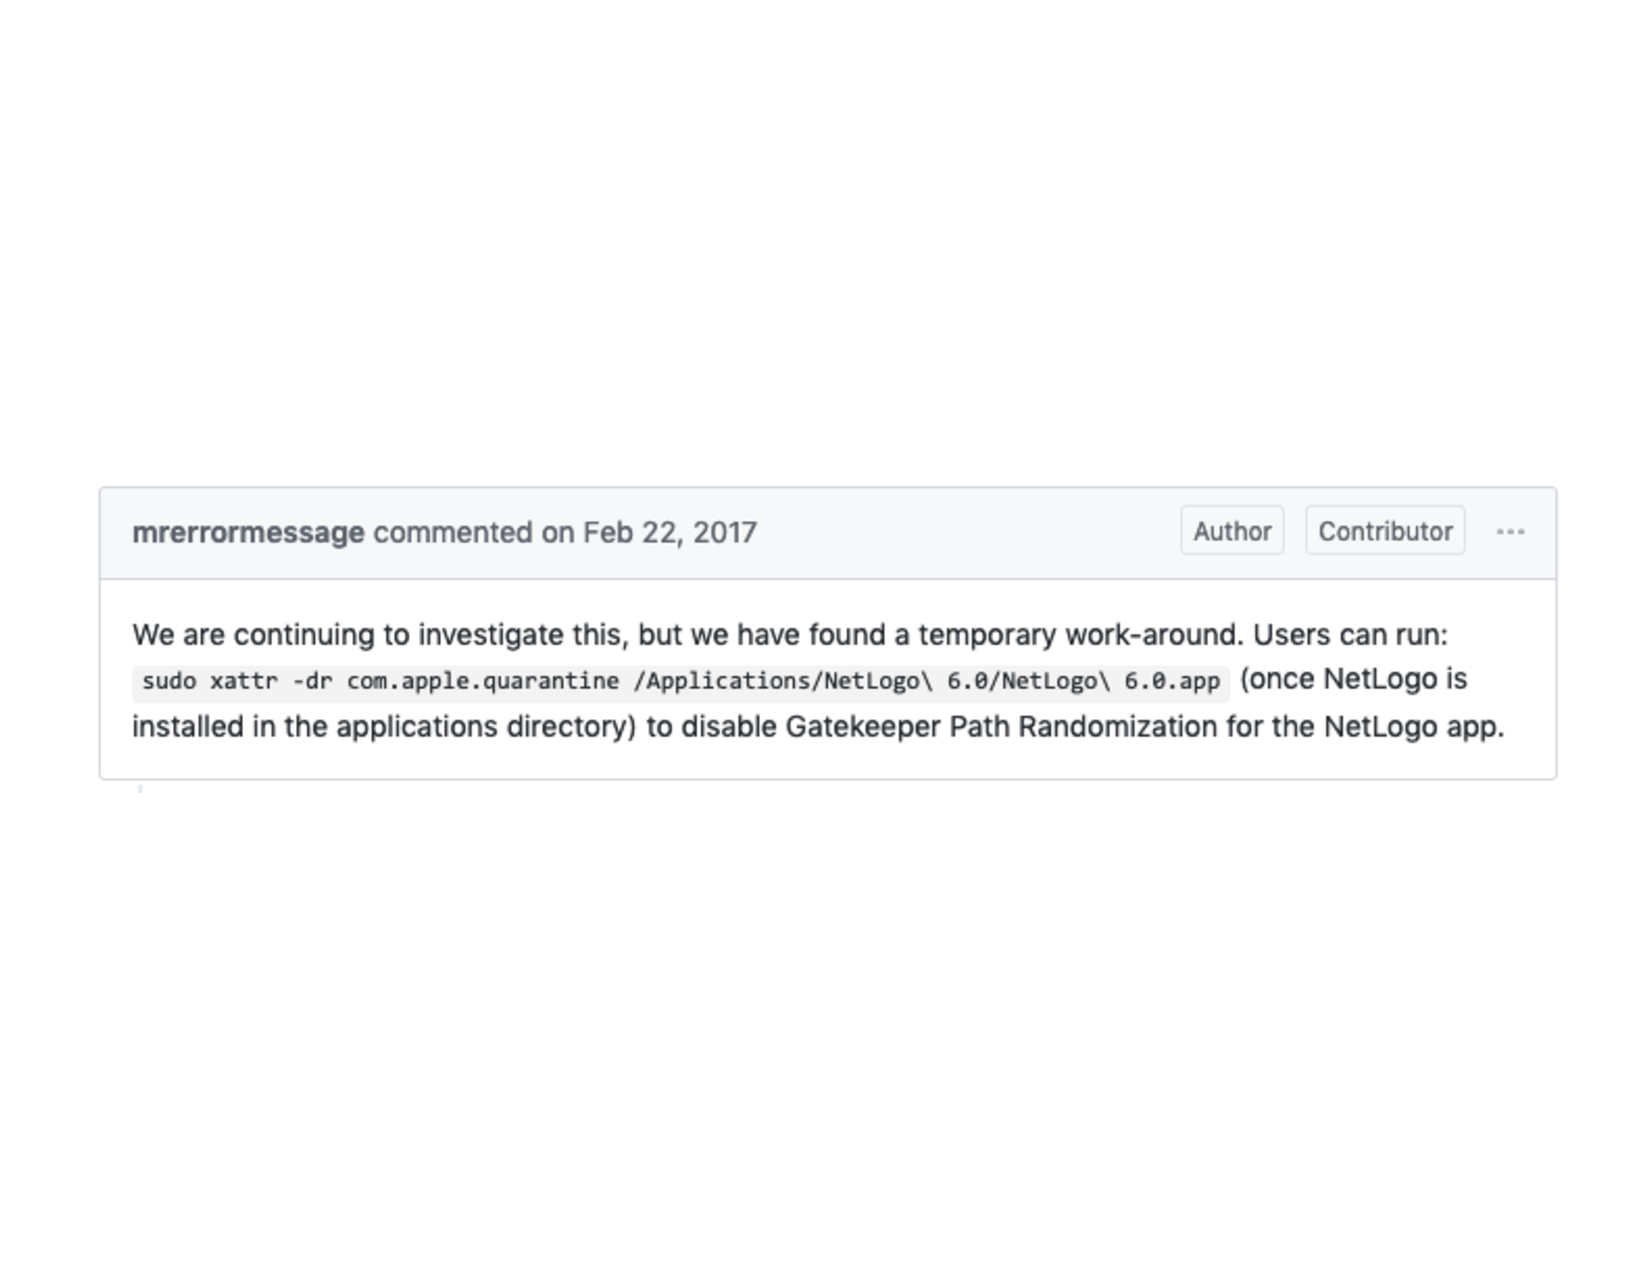
\includegraphics[height=3cm]{workaround}
\end{figure}

\texttt{RNetLogo} is also dependent on the package \texttt{rjava}. I continued to have problems related to my specific operating system and the \texttt{rjava} package, in a workshop setting with many different types of laptops it would not be possible to troubleshoot problems, so I had to abandoned \texttt{RNetLogo}. Later, on twitter the recommendation was made to use the package \texttt{nlrx}, but at this point, the Netlogo to R connection is only a minor component of the necessary work and I decided to work with each software separately rather spend more time on automating the crosstalk between \texttt{R} and \texttt{NetLogo}.

A limitation of \texttt{NetLogo} is that every event is scheduled per iteration/time step, however, the Gillespie algorithm requires that the next event occur after variable amounts of time and this issue is discussed in \citealt{Warnke}. For \texttt{Netlogo} the recommendation was to install and work with the \texttt{time} extension \citep{time}. Details of how to install are available from \cite{time} (specifically, download, name `time? and drop into extensions folder). The examples related to the \texttt{time} extension for \texttt{Netlogo} do not work for my installation of \texttt{NetLogo 6.0.4}. The Netlogo examples from \cite{Warnke} did not work either due to the same issue. Next, I read that \texttt{BehaviorSpace} (necessary to output the results of the ABM from \texttt{NetLogo}) is not compatible with the \texttt{time} extension.

Following these issues, I decided to track time as a variable and export it with \texttt{BehaviorSpace} bypassing he need to use the \texttt{time} extension. The downside of this approach is that time is nonlinear. Specifically, the visualizations in \texttt{NetLogo} show time progressing linearly, but in actuality, the amount of time that has passed between events is not constant. I am happy with this approach as the only dependency is on \texttt{Netlogo}.

\subsection{Debugging in NetLogo}
I have yet to really figure out how to debug in \texttt{NetLogo}. My current approach is to write in lines of code to \texttt{show X} where \texttt{X} is a parameter or \texttt{ask turtle 1 show X} if \texttt{X} is a \texttt{turtles-own} property. These values will then print into the Command Center window of the \texttt{NetLogo} interface.

\begin{thebibliography}{10}
\bibitem[Grider, 2017]{soln} Grider, R (mrerrormessage). 2017. Ensure NetLogo will open in Mac OS X Sierra \#1302. \url{https://github.com/NetLogo/NetLogo/issues/1302}

\bibitem[Sheppard and Railsback, 2015]{time} Sheppard, C. J. R., S. Railsback, S. 2015. Time Extension for NetLogo (version 1.2). \url{https://github.com/colinsheppard/time}

 \bibitem[Warnke et al., 2016]{Warnke} Warnke, T., O. Rienhardt, A. Uhrmacher. 2016. Population-based CTMCS and agent-based models. Proceedings of the 2016 Winter Simulation Conference. \url{https://ccl.northwestern.edu/2017/6.pdf}
 
\end{thebibliography}


\end{document}  